% !TEX program = xelatex
\documentclass[12pt,a4paper,fontset=fandol]{ctexart}
\usepackage[left=22mm,right=22mm,top=22mm,bottom=22mm]{geometry}
\usepackage{amsmath,amssymb,bm,mathtools}
\usepackage{graphicx,xcolor,booktabs,longtable,array,calc}
\usepackage{tikz}
\usetikzlibrary{arrows.meta,calc,decorations.pathmorphing}
\usepackage{setspace,enumitem,fancyhdr}
\usepackage[unicode,hidelinks]{hyperref}
\setstretch{1.24}
\setlength{\parindent}{2em}
\setlength{\parskip}{.35em}
\setlength{\emergencystretch}{2em}
\setlist{nosep,leftmargin=2em}
\setcounter{secnumdepth}{-1}
\ctexset{section={format=\Large\bfseries,beforeskip=1em,afterskip=.7em},
subsection={format=\large\bfseries,beforeskip=.8em,afterskip=.4em},
subsubsection={format=\normalsize\bfseries,beforeskip=.7em,afterskip=.3em}}
\allowdisplaybreaks[2]
\tikzset{arr/.style={-{Stealth[length=2mm]},semithick},
dot/.style={circle,fill,inner sep=1.5pt}}
\providecommand{\tightlist}{\setlength{\itemsep}{0pt}\setlength{\parskip}{0pt}}
\providecommand{\pandocbounded}[1]{#1}
\newsavebox{\diagrambox}
\pagestyle{fancy}
\fancyhf{}
\renewcommand{\headrulewidth}{0pt}
\fancyfoot[C]{\small \thepage}
\setlength{\headheight}{16pt}
\begin{document}
\begin{titlepage}
\thispagestyle{empty}
\vspace*{27mm}
\begin{center}
{\LARGE\bfseries 第39届全国中学生物理竞赛\par}
\vspace{8mm}
{\LARGE\bfseries 复赛理论试题\par}
\vspace{17mm}
{\Large 学生详解版\par}
\end{center}
\vfill
\end{titlepage}
\setcounter{page}{1}
\section{第 1
题　迈克尔逊干涉与液体折射率（40分）}\label{ux7b2c-1-ux9898-ux8fc8ux514bux5c14ux900aux5e72ux6d89ux4e0eux6db2ux4f53ux6298ux5c04ux738740ux5206}

迈克尔逊干涉仪的入射单色激光经过半反半透镜，分成沿两个互相垂直的臂传播的光束。分光片与入射光轴成\(45^\circ\)。臂端反射镜均垂直于相应臂，并能沿臂平移。返回的两束光在空间重叠而发生干涉。照明光为发散光时，观察到同心圆环。

分光片是在平整石英基板上蒸镀薄金属膜制成。两束参与叠加的光均在分光片反射一次，但分别在石英---金属、空气---金属界面反射；两种反射的相位突变之差记为\(\Delta\varphi\)。

\begin{center}
\begin{minipage}{\linewidth}
\centering\begingroup\sbox{\diagrambox}{\small
\begin{tikzpicture}[scale=1]
\draw[arr,blue] (-3,0)--(-.15,0); \node[above] at (-2.3,0) {发散激光};
\draw[very thick] (-.55,-.55)--(.55,.55); \node[below right] at (.6,-.5) {分光片};
\draw[arr,blue] (0,.1)--(0,2.4); \draw[arr,blue] (.12,2.4)--(.12,.2);
\draw[very thick] (-.7,2.5)--(.7,2.5); \node[above] at (0,2.6) {$M_1$};
\draw[arr,red] (.15,0)--(3,0); \draw[arr,red] (3,-.12)--(.2,-.12);
\draw[very thick] (3.1,-.7)--(3.1,.7); \node[right] at (3.2,.5) {$M_2$};
\draw[arr] (0,-.2)--(0,-2); \node[below] at (0,-2) {观察方向};
\draw[<->] (3.8,-.45)--(4.6,-.45); \node at (4.2,-.9) {平移};
\end{tikzpicture}
}
\ifdim\wd\diagrambox>.88\linewidth
\sbox{\diagrambox}{\resizebox{.88\linewidth}{!}{\usebox{\diagrambox}}}\fi
\ifdim\ht\diagrambox>.38\textheight
\resizebox{!}{.38\textheight}{\usebox{\diagrambox}}
\else\usebox{\diagrambox}\fi
\par\smallskip{\small 图1a　两臂光路及反射镜的平移方向\par}\endgroup\end{minipage}\end{center}

开始时，干涉场中心为亮斑，最外侧为亮圆环，计及中心共20个亮条纹。缓慢平移一个臂的反射镜，发现圆环越来越稀疏；中心明暗变化23个周期，视场最外侧变化20个周期。条纹计数均视为精确值，两臂长度在厘米量级。

（1）求\(\Delta\varphi\)。

（2）移动后可观察到多少个亮条纹，计及中心亮斑？

（3）将扁平石英空槽插入一臂，使槽表面垂直于臂。把槽倾斜\(\theta=5.00^\circ\)时，中心变化10个周期。注入待测液体后，再将槽恢复到垂直于臂，中心变化17个周期。光波长\(\lambda=633\,\mathrm{nm}\)，槽内壁间距\(t=2.00\,\mathrm{mm}\)，空气折射率1.00。求液体折射率。

\begin{center}
\begin{minipage}{\linewidth}
\centering\begingroup\sbox{\diagrambox}{\small
\begin{tikzpicture}[scale=1]
\draw[fill=blue!6] (0,0) rectangle(5,-1.7);
\coordinate (O) at (1,0); \coordinate (B) at (2.15,-1.7);
\draw[arr] (-.4,1.4)--(O); \draw[arr] (O)--(B); \draw[arr] (B)--(3.55,-3.1);
\draw[dashed] (1,1.35)--(1,-2.4); \draw[dashed] (2.15,-1.2)--(2.15,-2.8);
\draw (1,.7) arc(90:135:.7); \node at (.65,.85) {$\theta$};
\node at (1.28,-.65) {$i$}; \node at (4,-.8) {$n$};
\draw[<->] (5.35,0)--(5.35,-1.7) node[midway,right] {$t$};
\node at (2.4,1.85) {平行液层：$\sin\theta=n\sin i$};
\node at (2.4,-3.55) {须比较同一出射波前，不能只比较斜程};
\end{tikzpicture}
}
\ifdim\wd\diagrambox>.88\linewidth
\sbox{\diagrambox}{\resizebox{.88\linewidth}{!}{\usebox{\diagrambox}}}\fi
\ifdim\ht\diagrambox>.38\textheight
\resizebox{!}{.38\textheight}{\usebox{\diagrambox}}
\else\usebox{\diagrambox}\fi
\par\smallskip{\small 图1b　倾斜平行液层的折射几何\par}\endgroup\end{minipage}\end{center}

\subsection{一、题型定位}\label{ux4e00ux9898ux578bux5b9aux4f4d}

这是``用干涉计数反演相位与介质参数''的题。前两问属于等倾干涉：观察方向决定两束光的光程差，中心和边缘是两种不同的角度采样。第三问属于平行介质层的转角测量：必须比较同一出射波前，并把石英壁的贡献消去。

计算可从三个条纹计数入手：初态20条、中心变化23周期、边缘变化20周期。中心的计数直接测出镜子位移；边缘与中心计数之比测出视场角；初态条纹数再给出两臂的光学长度差。求出这些量后，可将亮纹条件按整周期取余，确定反射相位。

解题时要分清``观察到多少条亮纹''和``两个亮纹之间相差多少级''。中心与边缘都亮，20条亮纹对应19个完整级次间隔；移动后的计数也必须最后加1。

\subsection{二、知识点}\label{ux4e8cux77e5ux8bc6ux70b9}

\subsubsection{1.
等倾干涉的相位}\label{ux7b49ux503eux5e72ux6d89ux7684ux76f8ux4f4d}

将两臂返回光的几何等效为两平行反射面，设其初始光学长度差为\(d>0\)，观察倾角为\(\gamma\)。本题沿用参考解答的有向相位约定：

\[
\delta(\gamma)=\frac{4\pi d}{\lambda}\cos\gamma+\Delta\varphi.
\]

中心对应\(\gamma=0\)。亮纹条件是\(\delta=2\pi k\)，其中\(k\)为整数。光程差是\(2d\cos\gamma\)，系数2来自往返传播，不能把镜面移动量直接当作光程改变。

相位差的绝对符号依赖于把哪一束光减去哪一束；本题在上述约定下报告\(\Delta\varphi\)。可观测相位以\(2\pi\)为周期，因此最后只能确定模\(2\pi\)的结果。

\subsubsection{2.
镜面平移的计数}\label{ux955cux9762ux5e73ux79fbux7684ux8ba1ux6570}

镜面沿臂移动\(\Delta d\)，中心相位改变的绝对值为\(4\pi\Delta d/\lambda\)。若中心经历\(C\)个周期，则

\[
\Delta d=\frac{C\lambda}{2}.
\]

固定视场角\(\gamma_M\)处经历\(E\)个周期，则

\[
E=\frac{2\Delta d}{\lambda}\cos\gamma_M,
\qquad \cos\gamma_M=\frac EC.
\]

只在镜面始终垂直于臂、观察边缘角度不随调节改变时，这个比值才成立。若镜面同时倾斜，等倾条纹形态会改变，不能直接套用。

\subsubsection{3.
平行板的光程比较}\label{ux5e73ux884cux677fux7684ux5149ux7a0bux6bd4ux8f83}

对于折射率\(n\)、法向厚度\(t\)的平行液层，斯涅尔定律给出

\[
\sin\theta=n\sin i.
\]

光在液体中的单程长度为\(t/\cos i\)。但比较有液体与空气的两束光时，出射点发生横移；需要扣除传播到同一波前所对应的空气段。扣除后，单程光程增量是

\[
t(n\cos i-\cos\theta)
=t\left(\sqrt{n^2-\sin^2\theta}-\cos\theta\right).
\]

本题光往返穿越液层，故该式乘2。这个表达式具有两个立即可检验的极限：\(n=1\)时为零；\(\theta=0\)时为\(2t(n-1)\)。

\subsection{三、物理图像}\label{ux4e09ux7269ux7406ux56feux50cf}

镜子移动后环纹变稀，说明同一视场内能够容纳的级次跨度减少。在本题的正\(d\)约定下，光学长度差从\(d\)降为\(d-\Delta d\)。中心和边缘的相位都减小，但中心减得更快：中心减23级，边缘只减20级，所以二者级次差恰好减少3。

\begin{center}
\begin{minipage}{\linewidth}
\centering\begingroup\sbox{\diagrambox}{\small
\begin{tikzpicture}[scale=.75]
\foreach \rad in {.5,.85,1.13,1.4,1.67,1.9}{\draw (0,0) circle(\rad);}
\fill (0,0) circle(2pt); \node at (0,-2.45) {初态：20条亮纹};
\foreach \rad in {.6,1.02,1.4,1.74,1.9}{\draw (6,0) circle(\rad);}
\fill (6,0) circle(2pt); \node at (6,-2.45) {末态：17条亮纹};
\draw[arr] (2.25,0)--(3.75,0);
\node[align=center] at (3,1.35) {$d$减小\\视场固定};
\node at (3,-3.1) {示意只画部分环；计数使用中心到边缘的级次跨度};
\end{tikzpicture}
}
\ifdim\wd\diagrambox>.88\linewidth
\sbox{\diagrambox}{\resizebox{.88\linewidth}{!}{\usebox{\diagrambox}}}\fi
\ifdim\ht\diagrambox>.38\textheight
\resizebox{!}{.38\textheight}{\usebox{\diagrambox}}
\else\usebox{\diagrambox}\fi
\par\smallskip{\small 图1c　固定视场中环纹级次跨度的变化\par}\endgroup\end{minipage}\end{center}

图中只画了部分环。真正用于计算的是初态19个级次间隔和末态16个级次间隔。环纹``向内或向外移动''的视觉描述容易受观察方式影响，中心与边缘相位差的变化则不依赖这种描述。

第三问先测空槽，是为了校准槽壁引起的光程变化。空槽壁由石英组成，转动也会改变其光程。空槽的10周期就是石英壁的实验校准；装液后的17周期包含石英壁和液体的共同作用。只要石英壁几何、转动角度和往返路径保持一致，两次相位变化相减就消掉槽壁。

两次转动方向相反。因此不能把两次``周期数''未经定向就相加。先把两次变化都换成``从正放转到倾斜''的相位增量，再相减，液层相对于空气的转角贡献对应\(17-10=7\)周期。

\subsection{四、解题入口}\label{ux56dbux89e3ux9898ux5165ux53e3}

先写中心和视场边缘的亮纹条件，然后相减；不要先猜反射相位一定是\(\pi\)。金属膜两侧的反射相位并不能由``疏到密反射''一句话给定。

\[
\begin{aligned}
\frac{2d}{\lambda}+\frac{\Delta\varphi}{2\pi}&=k,\\
\frac{2d\cos\gamma_M}{\lambda}
+\frac{\Delta\varphi}{2\pi}&=k-19.
\end{aligned}
\]

两式之差消掉未知相位，得到\(d\)与\(\gamma_M\)的关系。另用23和20确定\(\gamma_M\)，方程便闭合。第三问另起一套光程模型，前两问求出的\(d\)不需要带入。

计算前统一单位：\(t=2.00\times10^{-3}\,\mathrm m\)，\(\lambda=6.33\times10^{-7}\,\mathrm m\)。角度进入数值三角函数时要确认采用角度制或先换成弧度。

\subsection{五、解析}\label{ux4e94ux89e3ux6790}

\subsubsection{（1）用三个整数确定反射相位}\label{ux7528ux4e09ux4e2aux6574ux6570ux786eux5b9aux53cdux5c04ux76f8ux4f4d}

设最大观察倾角为\(\gamma_M\)。初态中心和边缘之间相差19级：

\[
\frac{2d}{\lambda}(1-\cos\gamma_M)=19.
\]

中心与边缘的周期计数分别给出

\[
\frac{2\Delta d}{\lambda}=23,
\qquad
\frac{2\Delta d}{\lambda}\cos\gamma_M=20.
\]

所以

\[
\cos\gamma_M=\frac{20}{23},
\qquad \Delta d=\frac{23}{2}\lambda.
\]

代回初态级差：

\[
\frac{2d}{\lambda}
=\frac{19}{1-20/23}
=\frac{437}{3}=145+\frac23.
\]

中心亮纹要求\(2d/\lambda+\Delta\varphi/(2\pi)\)为整数。因此

\[
\boxed{\Delta\varphi=\frac{2\pi}{3}\pmod{2\pi}}.
\]

若取\(0\leq\Delta\varphi<2\pi\)，唯一代表值为\(2\pi/3\)；一般可写\(2\pi/3+2q\pi\)，\(q\in\mathbb Z\)。检验：取中心级次\(k=146\)，边缘级次为127，正好相差19。

这里求出的\(d=437\lambda/6\approx46.10\,\mu\mathrm m\)是两臂光学长度之差，完全可以远小于每条臂的厘米量级长度。不能因为题面说``臂长在厘米量级''，便把\(d\)强行取成厘米量级。

\subsubsection{（2）从级次差恢复条纹数}\label{ux4eceux7ea7ux6b21ux5deeux6062ux590dux6761ux7eb9ux6570}

环纹变稀使\(d\)减小。末态中心仍亮，因为其相位减少了整数23周期；最外侧也仍亮，因为其相位减少了整数20周期。

末态中心级次\(k'=k-23\)，边缘级次

\[
k'_M=(k-19)-20=k-39.
\]

故级次跨度为

\[
k'-k'_M=(k-23)-(k-39)=16.
\]

两端亮纹均计入，共

\[
\boxed{16+1=17\text{条亮纹}}.
\]

也可直接代入\(d'=d-\Delta d\)：

\[
\frac{2d'}{\lambda}(1-\cos\gamma_M)
=19-23\left(1-\frac{20}{23}\right)=16.
\]

两种算法一致。中心减少23级并不表示消失23条可见亮纹；可见条纹的变化取决于中心与边缘的相对变化，本题只少了3条。

\subsubsection{（3）建立液层的往返光程函数}\label{ux5efaux7acbux6db2ux5c42ux7684ux5f80ux8fd4ux5149ux7a0bux51fdux6570}

把``液体取代相同几何厚度的空气''的往返光程增量记为\(G(\theta)\)：

\[
G(\theta)=2t\left(\sqrt{n^2-\sin^2\theta}-\cos\theta\right).
\]

这里必须保留\(\cos\theta\)项。把空气段简单写成\(2t\)只在正入射时成立；在倾斜入射时这样做，会把空槽校准的物理含义丢掉。

为看清出射波前修正，可将图1b中的液体路径长度写成\(t/\cos i\)，相应空气等效路径写成

\[
\frac{t\cos(\theta-i)}{\cos i}.
\]

二者的光程差为

\[
\frac{t}{\cos i}\,[n-\cos(\theta-i)].
\]

利用\(\cos(\theta-i)=\cos\theta\cos i+\sin\theta\sin i\)，再用\(\sin\theta=n\sin i\)，该式化成\(t(n\cos i-\cos\theta)\)。乘2便得到\(G\)。

\subsubsection{消去槽壁并判断符号}\label{ux6d88ux53bbux69fdux58c1ux5e76ux5224ux65adux7b26ux53f7}

在角度从0到\(\theta\)的共同方向下，装液与空槽的相位变化之差等于\([G(\theta)-G(0)]/\lambda\)个周期。题面装液后实际从\(\theta\)转回0，周期数给的是变化的大小。参考光程方向下，两次校准相减得到

\[
G(\theta)-G(0)=(17-10)\lambda=7\lambda.
\]

等价地，

\[
2t\left[n-1-\sqrt{n^2-\sin^2\theta}
+\cos\theta\right]=-7\lambda.
\]

为什么右边是负值？对\(n>1\)且小\(\theta\)，\(G(\theta)\)比\(G(0)\)大。正放时液体造成的光程差虽很大，但本实验计数的是转角带来的小变化。必须避免把``填液产生很多条纹''和``填液后转动产生17周期''混为一谈。

\subsubsection{小角近似求折射率}\label{ux5c0fux89d2ux8fd1ux4f3cux6c42ux6298ux5c04ux7387}

仅对液体根号展开：

\[
\sqrt{n^2-\sin^2\theta}
=n-\frac{\sin^2\theta}{2n}
+O\!\left(\frac{\sin^4\theta}{n^3}\right).
\]

可得到

\[
\frac{t\sin^2\theta}{n}
-2t(1-\cos\theta)=-7\lambda.
\]

故

\[
n\simeq\frac{t\sin^2\theta}
{2t(1-\cos\theta)-7\lambda}.
\]

代入题给数据：

\[
\begin{aligned}
t\sin^25^\circ&=1.5192\times10^{-5}\,\mathrm m,\\
2t(1-\cos5^\circ)&=1.5221\times10^{-5}\,\mathrm m,\\
7\lambda&=4.431\times10^{-6}\,\mathrm m.
\end{aligned}
\]

由此\(n\simeq1.40797\)，按题给三位有效数字

\[
\boxed{n=1.41}.
\]

不展开根号而数值求解原方程，得\(n=1.40931\)，同样舍入为1.41。两者相差约\(0.096\%\)，本题报告精度下近似是足够的。保留这个对照有助于区分近似误差与单位错误。

\subsubsection{结果的物理与数量级检查}\label{ux7ed3ux679cux7684ux7269ux7406ux4e0eux6570ux91cfux7ea7ux68c0ux67e5}

由计数得到\(\gamma_M\simeq29.59^\circ\)。它未必是近轴小角，因此前两问使用精确\(\cos\gamma_M\)，没有对视场角展开。第三问的槽转角才是\(5.00^\circ\)，两个角属于不同几何，不能互相代换。

镜面位移为\(7.2795\,\mu\mathrm m\)，小于初始臂差\(46.10\,\mu\mathrm m\)，所以\(d\)没有越过零点，环纹变稀的方向解释一致。液体折射率大于1，空槽和装液的转角计数差为正，也与\(G(\theta)-G(0)>0\)相符。

还可用全小角形式理解测量灵敏度：

\[
7\lambda\simeq t\theta^2\left(1-\frac1n\right).
\]

光程变化随\(\theta^2\)变化。若转角非常小，计数只有不到一个周期，就难以用整数条纹精确反演折射率；若转角过大，则应回到根号形式，并检查光束横移是否超出有效口径。

\clearpage

\section{第 2
题　通电弹簧的平衡与稳定性（40分）}\label{ux7b2c-2-ux9898-ux901aux7535ux5f39ux7c27ux7684ux5e73ux8861ux4e0eux7a33ux5b9aux602740ux5206}

长直弹簧由涂绝缘漆的磷铜细丝绕制\(N\)匝，可视为半径\(r\)的长直螺线管。原长\(l_0\gg r\)，劲度系数\(k\)。形变时螺线管始终均匀密绕，半径变化可忽略。不计边缘效应、漏磁和重力，真空磁导率\(\mu_0\)。

（1）恒流源通过柔软导线给螺线管通以不变电流\(I_0\)，用外力使其无形变，随后缓慢撤除外力。新平衡长度\(l_p\)，弹簧仍可压缩或拉伸。

（i）导出可求\(l_p\)的代数方程，不必求解；求平衡附近小形变的等效弹性系数\(k_{\rm eff}\)，可含\(l_p\)。

（ii）求能实现平衡状态的\(I_0\)范围，不得含\(l_p\)。

（2）改用零电阻柔软导线把弹簧两端连接为闭合回路，并假设弹簧电阻也为零。初始电流\(I'_0\)，仍先用外力保持原长，再缓慢撤除。求新的平衡长度\(l'_p\)及等效弹性系数\(k'_{\rm eff}\)。

\begin{center}
\begin{minipage}{\linewidth}
\centering\begingroup\sbox{\diagrambox}{\small
\begin{tikzpicture}[scale=.9]
\draw[decorate,decoration={coil,aspect=.45,segment length=5mm,amplitude=4mm},thick] (0,0)--(6,0);
\draw[arr] (.2,-1)--(-1,-1) node[left] {$F_{\rm hold}$};
\draw[arr] (5.8,-1)--(7,-1) node[right] {$F_{\rm hold}$};
\draw[<->] (0,.9)--(6,.9) node[midway,above] {$l$};
\draw (0,0)--(0,-2)--(6,-2)--(6,0);
\draw[fill=white] (2.5,-2.4) rectangle(3.5,-1.6);
\node at (3,-2) {电路}; \node at (3,-2.95) {恒流源或理想闭合回路};
\node at (3,1.65) {$\mathcal L(l)=\mu_0\pi N^2r^2/l$};
\end{tikzpicture}
}
\ifdim\wd\diagrambox>.88\linewidth
\sbox{\diagrambox}{\resizebox{.88\linewidth}{!}{\usebox{\diagrambox}}}\fi
\ifdim\ht\diagrambox>.38\textheight
\resizebox{!}{.38\textheight}{\usebox{\diagrambox}}
\else\usebox{\diagrambox}\fi
\par\smallskip{\small 图2a　弹簧、保持力和两种供电约束\par}\endgroup\end{minipage}\end{center}

\subsection{一、题型定位}\label{ux4e00ux9898ux578bux5b9aux4f4d-1}

这是``电磁能量与力学势能耦合''的题。几何相同的弹簧，在恒流源和理想闭合回路中却有不同的电磁约束，因而有不同的平衡与刚度。

列能量关系前，应判断电流是否随线圈长度改变，并计入外部电源的功。恒流情况下，线圈压缩时电感增大，磁场储能增大，但电源同时向系统输送更多能量；用于求机械保持力的有效势能必须扣除这部分电源功。理想闭合回路没有电源，却因感应而保持磁通链不变。

本题第（1）（ii）还包含稳定性。代数方程有正根不等于缓慢撤除外力后可以稳定停住。先寻找平衡分支，再检查曲率，最后区分临界点和稳定分支，才能完整解释实验过程。

\subsection{二、知识点}\label{ux4e8cux77e5ux8bc6ux70b9-1}

\subsubsection{1.
电感取决于长度}\label{ux7535ux611fux53d6ux51b3ux4e8eux957fux5ea6}

螺线管内磁感应强度

\[
B=\mu_0\frac{NI}{l}.
\]

每匝磁通\(\Phi=B\pi r^2\)，总磁通链\(\Psi=N\Phi\)。为使符号清楚，令

\[
A=\mu_0\pi N^2r^2,\qquad
\mathcal L(l)=\frac{\Psi}{I}=\frac Al.
\]

这里\(A\)不是面积，具有``电感乘长度''的量纲。线圈截面积仍为\(\pi r^2\)。弹簧缩短时匝密度增大，电感随之增大。

\subsubsection{2.
磁场能和电源功}\label{ux78c1ux573aux80fdux548cux7535ux6e90ux529f}

磁场储能为

\[
W_B=\frac12\mathcal LI^2.
\]

若\(I=I_0\)不变，电源电压满足\(U=d(\mathcal LI_0)/dt\)，电源输入的微元功

\[
dW_{\rm src}=UI_0dt=I_0^2\,d\mathcal L.
\]

而磁场储能变化只有其一半：

\[
dW_B=\frac12I_0^2\,d\mathcal L.
\]

两者相减后的能量流向机械部分。这是恒流情况下不能直接对正磁能求导作为机械势能的原因。

\subsubsection{3.
保持力与恢复力}\label{ux4fddux6301ux529bux4e0eux6062ux590dux529b}

取长度增大的方向为广义正方向。缓慢改变长度所需外保持力满足

\[
F_{\rm hold}\,dl=dW_{\rm eff}.
\]

于是\(F_{\rm hold}=W'_{\rm eff}(l)\)。线圈自身的合广义力为其负值。平衡点要求\(F_{\rm hold}=0\)，附近

\[
F_{\rm hold}\simeq k_{\rm eff}\,\delta l,
\qquad k_{\rm eff}=W''_{\rm eff}(l_p).
\]

正刚度意味着自身力与位移方向相反。若二阶导数等于零，必须看更高阶项，不能直接断言中性稳定。

\subsection{三、物理图像}\label{ux4e09ux7269ux7406ux56feux50cf-1}

相邻同向电流匝相互吸引，电磁效应倾向使弹簧变短。弹簧被压缩后，弹性力倾向伸长。平衡是这两种趋势抵消。

恒流源使\(I\)不变，压缩会使\(B\propto1/l\)增大，电磁吸引随\(l^{-2}\)增强；这是一种使压缩继续加剧的反馈。如果电流过大，弹性恢复力无法产生稳定平衡。

理想闭合回路保持\(\Psi\)不变。压缩使\(\mathcal L\)增大，因此\(I\)反而减小，且\(I\propto l\)。于是\(B=\mu_0NI/l\)不变，电磁压缩力成为常量。在该理想模型里，它改变平衡位置，却不改变增量刚度。

\begin{center}
\begin{minipage}{\linewidth}
\centering\begingroup\sbox{\diagrambox}{\small
\begin{tikzpicture}[xscale=6,yscale=3]
\draw[arr] (0,0)--(1.13,0) node[right] {$x=l/l_0$};
\draw[arr] (0,0)--(0,1.18) node[above] {$I_0^2/I_c^2$};
\draw[thick,red,domain=.02:.66667,samples=70] plot(\x,{6.75*(1-\x)*\x*\x});
\draw[thick,blue,domain=.66667:1,samples=50] plot(\x,{6.75*(1-\x)*\x*\x});
\draw[dashed] (.66667,0)--(.66667,1)--(0,1);
\node[below] at (.66667,0) {$2/3$}; \node[left] at (0,1) {$1$};
\node[red] at (.3,.75) {不稳定}; \node[blue] at (.93,.95) {稳定};
\node at (.6,-.45) {峰顶是合并点，不是非线性稳定平衡};
\end{tikzpicture}
}
\ifdim\wd\diagrambox>.88\linewidth
\sbox{\diagrambox}{\resizebox{.88\linewidth}{!}{\usebox{\diagrambox}}}\fi
\ifdim\ht\diagrambox>.38\textheight
\resizebox{!}{.38\textheight}{\usebox{\diagrambox}}
\else\usebox{\diagrambox}\fi
\par\smallskip{\small 图2b　恒流平衡分支与临界点\par}\endgroup\end{minipage}\end{center}

图中横坐标是长度比，纵坐标是电流平方比。右侧蓝色分支连接\(I_0=0,l=l_0\)，缓慢增大电流时会沿此分支缩短。左侧红色分支虽满足力平衡，却对微扰不稳定。顶点是两分支合并的极限。

\subsection{四、解题入口}\label{ux56dbux89e3ux9898ux5165ux53e3-1}

第一步只做几何，写\(\mathcal L=A/l\)。第二步写约束：恒流源是\(I=I_0\)；理想闭合回路是\(\mathcal LI=\mathcal L_0I'_0\)。第三步把两种约束各自代入能量式。

恒流源情形，从能量守恒微元式

\[
F_{\rm hold}\,dl+dW_{\rm src}
=dW_{\rm el}+dW_B
\]

出发。闭合回路情形没有电源功，直接用弹性势能加磁能。两种情形应分开列式，不能先写一个总势能，再随意把\(I\)视作常量或变量。

为讨论范围，将恒流平衡方程变成\(I_0^2\)关于\(l_p\)的函数。这比直接解三次方程容易，因为一个函数最大值就能决定是否有正长度平衡。

\subsection{五、解析}\label{ux4e94ux89e3ux6790-1}

\subsubsection{（1）（i）恒流源下的有效势能}\label{iux6052ux6d41ux6e90ux4e0bux7684ux6709ux6548ux52bfux80fd}

弹性势能

\[
W_{\rm el}=\frac12k(l-l_0)^2.
\]

电源功微元与磁能微元相减，得到

\[
F_{\rm hold}\,dl
=d\left[\frac12k(l-l_0)^2
-\frac12\mathcal L(l)I_0^2\right].
\]

因此可用的机械有效势能为

\[
W_{\rm eff}(l)=\frac12k(l-l_0)^2-\frac{AI_0^2}{2l}.
\]

其负磁项并不意味着实际磁场能为负；它是计入恒流源能量交换后对机械运动起作用的势能。实际磁能仍是\(AI_0^2/(2l)>0\)。

对\(l\)求导：

\[
F_{\rm hold}=k(l-l_0)+\frac{AI_0^2}{2l^2}.
\]

撤去保持力时

\[
\boxed{k(l_p-l_0)+\frac{AI_0^2}{2l_p^2}=0}.
\]

也可写成多项式

\[
\boxed{l_p^3-l_0l_p^2+\frac{AI_0^2}{2k}=0}.
\]

当\(I_0\neq0\)，该式要求\(l_p<l_0\)，与电磁吸引导致压缩一致。初始无形变时需要的外力为\(AI_0^2/(2l_0^2)\)，方向是拉长弹簧，用以抵消磁吸引。

\subsubsection{小形变等效刚度}\label{ux5c0fux5f62ux53d8ux7b49ux6548ux521aux5ea6}

令\(l=l_p+\delta l\)，对保持力作一阶展开：

\[
F_{\rm hold}(l)
=F_{\rm hold}(l_p)
+\left(k-\frac{AI_0^2}{l_p^3}\right)\delta l
+O(\delta l^2).
\]

于是

\[
\boxed{k_{\rm eff}=k-\frac{AI_0^2}{l_p^3}}.
\]

利用平衡条件消去\(I_0\)，还可写为

\[
AI_0^2=2k(l_0-l_p)l_p^2,
\qquad
\boxed{k_{\rm eff}=k\,\frac{3l_p-2l_0}{l_p}}.
\]

两式各有用途：前式直接显示磁效应降低刚度；后式直接显示稳定分支要求\(l_p>2l_0/3\)。若给弹簧某个等效运动质量\(M\)，小振动频率便是\(\sqrt{k_{\rm eff}/M}\)，但本题没有给质量，不需要另求频率。

\subsubsection{（1）（ii）电流阈值与分支}\label{iiux7535ux6d41ux9608ux503cux4e0eux5206ux652f}

由平衡条件

\[
I_0^2=\frac{2k}{A}(l_0-l_p)l_p^2,
\qquad 0<l_p<l_0.
\]

令\(f(l)=(l_0-l)l^2\)。求导得

\[
f'(l)=l(2l_0-3l).
\]

它在\(l=2l_0/3\)达到唯一内部最大值：

\[
f_{\max}=\frac{4l_0^3}{27}.
\]

所以存在正长度平衡解的电流范围为

\[
\boxed{|I_0|\leq I_c,\qquad
I_c=\sqrt{\frac{8kl_0^3}{27\mu_0\pi N^2r^2}}}.
\]

若\(I_0\)指电流大小，则写\(0\leq I_0\leq I_c\)。电流反向不会改变磁能和匝间吸引，故阈值依赖平方。

在\(0<|I_0|<I_c\)时有两个正根：一个在\((0,2l_0/3)\)，另一个在\((2l_0/3,l_0)\)。前者\(k_{\rm eff}<0\)，后者\(k_{\rm eff}>0\)。缓慢撤去外力而要求可以停留的平衡，选择后者。

参考解答将临界等号包括在``能实现平衡''的代数范围里。若强调抗微扰的稳定平衡，则应进一步写

\[
\boxed{|I_0|<I_c,\qquad l_p>2l_0/3}.
\]

零电流时\(l_p=l_0\)，刚度为\(k\)，也属于稳定情形。

\subsubsection{临界点为什么不是稳定平台}\label{ux4e34ux754cux70b9ux4e3aux4ec0ux4e48ux4e0dux662fux7a33ux5b9aux5e73ux53f0}

临界电流时\(l_c=2l_0/3\)，\(W'_{\rm eff}(l_c)=W''_{\rm eff}(l_c)=0\)，但

\[
W'''_{\rm eff}(l_c)
=\frac{3AI_c^2}{l_c^4}>0.
\]

因此局部势能有非零三次项：

\[
W_{\rm eff}(l_c+\delta l)
-W_{\rm eff}(l_c)
\simeq\frac{W'''_{\rm eff}(l_c)}6\,\delta l^3.
\]

势能不是极小值。合机械力在两侧的最低阶项均指向缩短方向：稍微压缩后不会回到原点。它是稳定与不稳定分支合并的临界点，而不是一段平坦势阱。

对于\(|I_0|>I_c\)，在\(0<l<l_0\)范围内没有平衡根，模型预测持续压缩。然而\(l\)很小时长螺线管近似和``匝间仍能运动''的假设先失效，不能把数学上的\(l\to0\)当成真实弹簧结局。

\subsubsection{（2）闭合零电阻回路的守恒量}\label{ux95edux5408ux96f6ux7535ux963bux56deux8defux7684ux5b88ux6052ux91cf}

闭合回路中没有电阻、没有外加电动势，法拉第定律给出

\[
\frac{d\Psi}{dt}=0,
\qquad \Psi=\mathcal LI=\mathcal L_0I'_0.
\]

初始电感\(\mathcal L_0=A/l_0\)，因此

\[
\frac Al I=\frac A{l_0}I'_0,
\qquad \boxed{I(l)=I'_0\frac l{l_0}}.
\]

注意守恒的是所有匝的磁通链，不是电流。这里\(N\)固定，因此每匝磁通也固定；若匝数变化，两者不能混同。

\subsubsection{总势能与平衡长度}\label{ux603bux52bfux80fdux4e0eux5e73ux8861ux957fux5ea6}

在固定\(\Psi\)约束下，磁能为

\[
W'_B=\frac{\Psi^2}{2\mathcal L}
=\frac{A{I'_0}^2}{2l_0^2}\,l.
\]

于是没有电源功时的总势能

\[
W'(l)=\frac12k(l-l_0)^2
+\frac{A{I'_0}^2}{2l_0^2}\,l.
\]

保持力

\[
F'_{\rm hold}=k(l-l_0)
+\frac{A{I'_0}^2}{2l_0^2}.
\]

令其为零，得

\[
\boxed{l'_p=l_0-\frac{\mu_0\pi N^2r^2{I'_0}^2}{2kl_0^2}}.
\]

再求导可得

\[
\boxed{k'_{\rm eff}=k}.
\]

磁能是长度的一次函数，所以提供恒定压缩力，没有二阶曲率。这是两种供电方式差异的最简数学表达。

\subsubsection{适用条件与横向比较}\label{ux9002ux7528ux6761ux4ef6ux4e0eux6a2aux5411ux6bd4ux8f83}

要得到正长度，闭合回路初始电流需满足

\[
{I'_0}^2<\frac{2kl_0^3}{A}.
\]

还必须有\(l'_p\gg r\)，并且压缩未达到线圈接触或弹簧材料极限。题目假定``仍可压缩或拉伸''，正是排除接触锁死对刚度的干扰。

把两种模型在\(l=l_0\)附近作弱电流展开，其一阶平衡缩短量相同：

\[
l_0-l_p\simeq\frac{AI_0^2}{2kl_0^2},
\qquad
l_0-l'_p=\frac{A{I'_0}^2}{2kl_0^2}.
\]

但恒流刚度已经降低，闭合回路刚度仍为\(k\)。仅测一次平衡位移可能区分不了两种约束，测量小振动或增量力则能区分。

量纲检查也很有效：\(AI^2/l\)为能量；\(AI^2/l^2\)为力；\(AI^2/l^3\)为刚度。若答案中的磁刚度写成\(l^{-2}\)，一定遗漏了一次求导。

\clearpage

\section{第 3
题　实心球在粗糙斜面上的多次弹性碰撞（40分）}\label{ux7b2c-3-ux9898-ux5b9eux5fc3ux7403ux5728ux7c97ux7cd9ux659cux9762ux4e0aux7684ux591aux6b21ux5f39ux6027ux78b0ux649e40ux5206}

质量\(m\)、半径\(R\)的均匀实心球从倾角\(\theta\)的无限长固定斜面上发射，球心初速度垂直于斜面，大小\(V\)，初始自转角速度为零。建立斜面坐标系：\(x\)沿斜面向下，\(y\)垂直于斜面向上。

球与斜面碰撞是弹性的，碰撞时间极短，碰撞前后法向速度大小不变。斜面足够粗糙，碰撞时摩擦足够大、接触点无相对滑动。球绕直径的转动惯量为\(I=2mR^2/5\)。

\begin{center}
\begin{minipage}{\linewidth}
\centering\begingroup\sbox{\diagrambox}{\small
\begin{tikzpicture}[scale=.9]
\draw[thick] (-.8,0)--(8,0); \draw[arr] (0,0)--(8.4,0) node[right] {$x$};
\draw[arr] (0,0)--(0,3.5) node[above] {$y$};
\draw[thick,blue,domain=0:6,samples=80] plot(\x,{1.65*sqrt(\x)-.674*\x});
\draw[arr] (0,.3)--(0,1.25) node[left] {$V$};
\draw[arr] (2.5,3.1)--(3.6,1.8) node[right] {$\boldsymbol g$};
\node at (5,3.8) {$a_x=g\sin\theta,\quad a_y=-g\cos\theta$};
\node at (4,-.7) {每次离面法向速度相同，飞行时间均为$T$};
\end{tikzpicture}
}
\ifdim\wd\diagrambox>.88\linewidth
\sbox{\diagrambox}{\resizebox{.88\linewidth}{!}{\usebox{\diagrambox}}}\fi
\ifdim\ht\diagrambox>.38\textheight
\resizebox{!}{.38\textheight}{\usebox{\diagrambox}}
\else\usebox{\diagrambox}\fi
\par\smallskip{\small 图3a　斜面坐标下的飞行段\par}\endgroup\end{minipage}\end{center}

求：（1）第一次碰撞前球心速度和自转角速度；（2）第一次碰撞后两者；（3）第\(n\)次碰撞后球心沿\(x\)方向的速度和自转角速度；（4）前\(n\)次碰撞中斜面对球施加的总冲量。

\subsection{一、题型定位}\label{ux4e00ux9898ux578bux5b9aux4f4d-2}

本题将``连续飞行''和``瞬时碰撞''交替连接。飞行段由抛体运动控制，碰撞段由冲量、角冲量和弹性条件控制。先建立一次碰撞的输入---输出关系，再研究其重复，远比逐次计算方便。

难点是平动和自转交换能量。只对球心写动量定理不能确定碰撞后的两个未知量；只写动能守恒又不能确定摩擦冲量方向。角动量关系与能量守恒必须配合使用。

本稿采用与参考解答一致的``完全弹性粗糙接触''模型。题面``无相对滑动''描述碰撞接触过程的充分摩擦，并不等于脱离斜面后立即满足\(v_x=R\omega\)。若把刚性瞬时碰撞理解为强制碰后纯滚动，则一般会损失切向动能，与本题弹性条件不同。

\subsection{二、知识点}\label{ux4e8cux77e5ux8bc6ux70b9-2}

\subsubsection{1.
斜面坐标中的重力}\label{ux659cux9762ux5750ux6807ux4e2dux7684ux91cdux529b}

\[
a_x=g\sin\theta,\qquad a_y=-g\cos\theta.
\]

球心到斜面的距离为\(R\)，将其相对于接触高度的法向位移记为\(Y\)，则离面时\(Y(0)=0\)。各次飞行只需用这个相对位移，不需要把球心几何高度误写为零。

正常情形取\(0\leq\theta<\pi/2\)。法向抛起速度为\(V\)时，重返斜面的时间

\[
T=\frac{2V}{g\cos\theta}.
\]

每次碰撞后法向速度都为\(+V\)，所以每段飞行时间相同。每段飞行带来的切向速度增量也相同：

\[
w=gT\sin\theta=2V\tan\theta.
\]

\subsubsection{2.
自转符号与接触速度}\label{ux81eaux8f6cux7b26ux53f7ux4e0eux63a5ux89e6ux901fux5ea6}

顺时针自转取\(\omega>0\)，相应球底接触点的自转速度沿\(x\)负方向。接触点相对斜面的切向速度为

\[
u=v_x-R\omega.
\]

定义\(b=R\omega\)，使平动速度与自转变量有相同量纲。实心球的切向和转动动能是

\[
K_t=\frac12m\left(v_x^2+\frac25b^2\right).
\]

比较能量时不能把\(v_x^2+b^2\)直接相加；转动惯量系数\(2/5\)必须保留。

\subsubsection{3.
碰撞的冲量关系}\label{ux78b0ux649eux7684ux51b2ux91cfux5173ux7cfb}

设斜面对球的有向切向冲量为\(J_x\)，则

\[
m(v_f-v_i)=J_x,\qquad
I(\omega_f-\omega_i)=-RJ_x.
\]

所以

\[
v_f-v_i=-\frac25(b_f-b_i).
\]

等价于\(v+(2/5)b\)在一次碰撞中不变。这也可由关于接触点的角动量守恒推出：接触冲量对接触点力矩为零，重力冲量在极短碰撞时间内忽略。

\subsection{三、物理图像}\label{ux4e09ux7269ux7406ux56feux50cf-2}

球在空中仅受重力，重力通过球心，故自转角速度不变。沿斜面方向的速度每次增加\(w\)，为下一次碰撞提供新的切向输入。

第一次落到斜面时没有自转、球心向下滑。摩擦冲量向斜面上方，使球心切向速度减小并产生顺时针自转。弹性接触在压缩阶段储存能量，再在恢复阶段释放，所以碰后可能出现``自转比平动更快''的状态。

\begin{center}
\begin{minipage}{\linewidth}
\centering\begingroup\sbox{\diagrambox}{\small
\begin{tikzpicture}[scale=1]
\draw[thick] (-2,0)--(2,0); \draw[thick] (0,.8) circle(.8);
\fill (0,.8) circle(1.4pt); \fill (0,0) circle(1.4pt);
\draw[arr] (0,0)--(0,1.8) node[above] {$J_y$};
\draw[arr] (0,0)--(-1.4,0) node[below left] {$J_x$};
\draw[arr] (.3,.8)--(1.6,.8) node[right] {$v_x$};
\draw[arr] (.65,1.5) arc(45:-35:1); \node at (1.3,1.8) {$\omega>0$};
\node at (0,-.7) {顺时针取正，$u=v_x-R\omega$};
\end{tikzpicture}
}
\ifdim\wd\diagrambox>.88\linewidth
\sbox{\diagrambox}{\resizebox{.88\linewidth}{!}{\usebox{\diagrambox}}}\fi
\ifdim\ht\diagrambox>.38\textheight
\resizebox{!}{.38\textheight}{\usebox{\diagrambox}}
\else\usebox{\diagrambox}\fi
\par\smallskip{\small 图3b　碰撞冲量及顺时针自转约定\par}\endgroup\end{minipage}\end{center}

从公式将看到，完全弹性粗糙碰撞使\(u_f=-u_i\)。第一次碰后\(u<0\)，第二次飞行让\(v_x\)增加\(w\)，再经一次碰撞后恰好有\(u=0\)。奇数、偶数次的结果不同，源头是接触相对速度的翻转，而不是任意的代数符号。

碰撞所说的``无滑动''必须结合有限形变理解：真实接触区可以有弹性切向形变而无滑移，分离瞬间的刚体速度仍可改变符号。本题简化为能量无损的粗糙弹性映射。若改用切向完全非弹性粘着模型，碰后\(u=0\)，答案将改变，后面的变式给出这种对照。

\subsection{四、解题入口}\label{ux56dbux89e3ux9898ux5165ux53e3-2}

用\(v_n\)表示第\(n\)次碰后的切向球心速度，用\(b_n=R\omega_n\)表示同时刻自转变量，初始\(v_0=b_0=0\)。第\(n\)次碰前是

\[
(v_n^-,b_n^-)=(v_{n-1}+w,b_{n-1}).
\]

只需先求一次碰撞算子

\[
(v_i,b_i)\longmapsto(v_f,b_f).
\]

然后寻找两种线性组合：一个碰撞时不变，另一个碰撞时变号。这样可以把二元耦合递推拆成两条标量递推，分别求解后还原\(v_n,b_n\)。

总冲量应在最后求。每一次冲量单独列出来容易产生复杂求和；使用动量变化减去飞行阶段重力冲量，可直接得到望远镜求和。

\subsection{五、解析}\label{ux4e94ux89e3ux6790-2}

\subsubsection{（1）第一次碰撞前}\label{ux7b2cux4e00ux6b21ux78b0ux649eux524d}

以发射时为\(t=0\)，相对接触高度的运动方程为

\[
Y(t)=Vt-\frac12g\cos\theta\,t^2,
\qquad x(t)=\frac12g\sin\theta\,t^2.
\]

再次到达\(Y=0\)的非零时刻是\(T=2V/(g\cos\theta)\)。因而

\[
v_x^-=gT\sin\theta=w=2V\tan\theta,
\qquad v_y^-=V-gT\cos\theta=-V.
\]

空中重力关于球心的力矩为零，故

\[
\boxed{\boldsymbol v_1^-
=2V\tan\theta\,\hat{\boldsymbol x}
-V\,\hat{\boldsymbol y},\qquad\omega_1^-=0}.
\]

该段切向位移为\(g\sin\theta\,T^2/2\)。本题未要求落点，但这一结果能检验\(x\)正方向是否选对。

\subsubsection{（2）先求一般粗糙弹性碰撞}\label{ux5148ux6c42ux4e00ux822cux7c97ux7cd9ux5f39ux6027ux78b0ux649e}

法向速度反号而大小不变，故法向动能前后相同。弹性条件可单独写在切向---自转部分：

\[
v_f^2+\frac25b_f^2
=v_i^2+\frac25b_i^2.
\]

冲量关系是

\[
v_f-v_i=-\frac25(b_f-b_i).
\]

将能量式分解：

\[
(v_f-v_i)(v_f+v_i)
+\frac25(b_f-b_i)(b_f+b_i)=0.
\]

若碰撞有非零切向冲量，利用前式消去差量，得

\[
v_f+v_i=b_f+b_i,
\]

即\(u_f=-u_i\)。联立两线性关系，得到

\[
\boxed{
\begin{aligned}
v_f&=\frac37v_i+\frac47b_i,\\
b_f&=\frac{10}{7}v_i-\frac37b_i.
\end{aligned}}
\]

若本来\(u_i=0\)，非零冲量分支与零冲量分支重合，映射仍给\(v_f=v_i,b_f=b_i\)。因此无需另加一条不连续规则。

\subsubsection{第一次碰后结果}\label{ux7b2cux4e00ux6b21ux78b0ux540eux7ed3ux679c}

代\(v_i=w,b_i=0\)：

\[
v_1=\frac37w,\qquad
b_1=\frac{10}{7}w.
\]

法向速度为\(+V\)，所以

\[
\boxed{
\boldsymbol v_1^+
=\frac67V\tan\theta\,\hat{\boldsymbol x}
+V\,\hat{\boldsymbol y}},
\]

\[
\boxed{\omega_1^+=\frac{20V\tan\theta}{7R}}
\quad\text{（顺时针）}.
\]

第一次切向冲量

\[
J_{x,1}=m(v_1-w)=-\frac47mw,
\]

法向冲量\(J_{y,1}=2mV\)。负的\(J_x\)与图中向斜面上方的摩擦一致。

能量检验：

\[
\left(\frac37w\right)^2
+\frac25\left(\frac{10}{7}w\right)^2
=\frac9{49}w^2+\frac{40}{49}w^2=w^2.
\]

因此虽球心切向速度减小，切向总动能没有损失；减小的部分进入自转。

\subsubsection{（3）二元递推方程}\label{ux4e8cux5143ux9012ux63a8ux65b9ux7a0b}

第\(n\)次碰撞前，飞行使\(v_{n-1}\)增加\(w\)，自转不变。故

\[
\begin{aligned}
v_n&=\frac37(v_{n-1}+w)+\frac47b_{n-1},\\
b_n&=\frac{10}{7}(v_{n-1}+w)-\frac37b_{n-1}.
\end{aligned}
\]

注意\(w\)必须只加在碰前平动速度中。将其同时加到\(b\)，相当于错误地认为重力会使球自转加速。

定义

\[
u_n=v_n-b_n,\qquad
z_n=v_n+\frac25b_n.
\]

则递推分别变为

\[
u_n=-u_{n-1}-w,
\qquad z_n=z_{n-1}+w.
\]

\(u_0=z_0=0\)，所以

\[
u_n=\frac{(-1)^n-1}{2}w,
\qquad z_n=nw.
\]

第一条可用前两项看出：\(u_1=-w,u_2=0,u_3=-w\)。第二条是等差数列。

\subsubsection{还原平动与自转}\label{ux8fd8ux539fux5e73ux52a8ux4e0eux81eaux8f6c}

由\(z_n=u_n+(7/5)b_n\)，

\[
b_n=\frac57(z_n-u_n),
\qquad
v_n=\frac57z_n+\frac27u_n.
\]

因此统一形式为

\[
\boxed{v_n=\frac{5n+(-1)^n-1}{7}w},
\]

\[
\boxed{
\omega_n=\frac{5}{7R}
\left[n+\frac{1-(-1)^n}{2}\right]w}.
\]

代\(w=2V\tan\theta\)后，偶数\(n\)有

\[
\boxed{v_n=\frac{10n}{7}V\tan\theta,\qquad
\omega_n=\frac{10n}{7R}V\tan\theta}.
\]

奇数\(n\)有

\[
\boxed{v_n=\frac{2(5n-2)}7V\tan\theta,\qquad
\omega_n=\frac{10(n+1)}{7R}V\tan\theta}.
\]

法向碰后速度始终为\(V\)。\(n=1\)恢复前一问；\(n=2\)给\(v_2=b_2=10w/7\)，刚好纯滚动速度关系；\(n=3\)给\(v_3=13w/7,b_3=20w/7\)。

\subsubsection{两次碰撞一组的解法}\label{ux4e24ux6b21ux78b0ux649eux4e00ux7ec4ux7684ux89e3ux6cd5}

一次碰撞矩阵

\[
M=\frac17
\begin{pmatrix}3&4\\10&-3\end{pmatrix}
\]

满足\(M^2=\mathbf1\)。一段飞行的增量向量为\(\boldsymbol a=(w,0)^{\mathsf T}\)，于是

\[
\boldsymbol q_n=M(\boldsymbol q_{n-1}+\boldsymbol a),
\quad
\boldsymbol q_{n+2}=\boldsymbol q_n+(\mathbf1+M)\boldsymbol a.
\]

而

\[
(\mathbf1+M)\boldsymbol a
=\frac{10w}{7}\begin{pmatrix}1\\1\end{pmatrix}.
\]

每两次碰后，平动和自转变量都增加\(10w/7\)。从\((0,0)\)和\((3w/7,10w/7)\)两个起点即可分别得到偶、奇数序列。这个方法直接揭示周期翻转与线性增长共存。

\subsubsection{\texorpdfstring{（4）前\(n\)次总冲量}{（4）前n次总冲量}}\label{ux524dnux6b21ux603bux51b2ux91cf}

第\(j\)次碰撞的切向冲量是

\[
J_{x,j}=m[v_j-(v_{j-1}+w)].
\]

求和时中间速度相消：

\[
J_x=m(v_n-v_0)-nmw=m(v_n-nw).
\]

因此

\[
J_x=-\frac{mw}{7}[2n+1-(-1)^n].
\]

每次法向冲量相同，故

\[
J_y=\sum_{j=1}^n2mV=2nmV.
\]

总冲量统一写成

\[
\boxed{
\boldsymbol J=\frac{2mV}{7}
\left\{-[2n+1-(-1)^n]\tan\theta\,
\hat{\boldsymbol x}+7n\,\hat{\boldsymbol y}\right\}}.
\]

偶数\(n\)时

\[
\boldsymbol J=\frac{2nmV}{7}
(-2\tan\theta\,\hat{\boldsymbol x}+7\hat{\boldsymbol y});
\]

奇数\(n\)时

\[
\boldsymbol J=\frac{2nmV}{7}
\left[-2\left(1+\frac1n\right)\tan\theta\,
\hat{\boldsymbol x}+7\hat{\boldsymbol y}\right].
\]

这里求的是碰撞过程中斜面的冲量，未包含飞行阶段重力冲量。如果直接用总动量差当斜面冲量，\(x\)方向会漏减\(nmw\)，\(y\)方向也会漏计飞行中的重力作用。

\par\noindent\begin{minipage}{\linewidth}
\subsubsection{奇偶结构的进一步检验}\label{ux5947ux5076ux7ed3ux6784ux7684ux8fdbux4e00ux6b65ux68c0ux9a8c}

当偶数\(n\)碰后有\(u_n=0\)，随后飞行使碰前\(u^-_{n+1}=w\)，下一次切向冲量为\(-4mw/7\)。奇数\(n\)碰后有\(u_n=-w\)，下一段飞行使\(u^-_{n+1}=0\)，因此下一次碰撞切向冲量为零。

所以只有奇数次碰撞有切向冲量：

\[
J_x=-\frac47mw\,\left\lceil\frac n2\right\rceil.
\]

它与上面的统一式完全一致。每次都可能存在法向冲量，但有法向碰撞不意味着一定有摩擦冲量。

\(\theta=0\)时\(w=0\)，所有切向速度和自转为零，只做法向弹跳，总冲量为\(2nmV\hat{\boldsymbol y}\)。\(R\)只影响角速度，不影响\(b=R\omega\)和平动结果，符合相似尺寸球在同一质量分布系数下的碰撞缩放。

\end{minipage}\par
\clearpage

\section{第 4
题　随圆环转动的铰接细杆（60分）}\label{ux7b2c-4-ux9898-ux968fux5706ux73afux8f6cux52a8ux7684ux94f0ux63a5ux7ec6ux674660ux5206}

匀质刚性细杆长\(2a\)、质量\(m\)，一端小孔嵌套在半径\(R\)的水平圆环的固定点\(P\)。\(P\)随圆环绕中心竖直轴以恒定角速度\(\omega\)转动；杆同时可绕\(P\)无摩擦转动，且杆与矢径\(OP\)始终在同一竖直平面内。杆与竖直向上方向的夹角为\(\theta\)，由竖直向上转向径向外侧的方向为正，重力加速度\(g\)。

\begin{center}
\begin{minipage}{\linewidth}
\centering\begingroup\sbox{\diagrambox}{\small
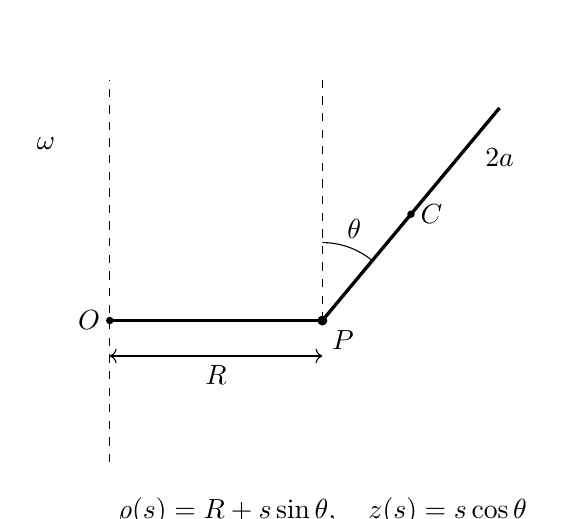
\begin{tikzpicture}[scale=.9]
\draw[dashed] (-3,-2)--(-3,3.4); \fill (-3,0) circle(1.5pt) node[left] {$O$};
\draw[thick] (-3,0)--(0,0); \fill (0,0) circle(2pt) node[below right] {$P$};
\draw[very thick] (0,0)--(2.5,3);
\draw[dashed] (0,0)--(0,3.5);
\draw (0,1.1) arc(90:50.2:1.1); \node at (.45,1.3) {$\theta$};
\fill (1.25,1.5) circle(1.5pt) node[right] {$C$};
\draw[<->] (-3,-.5)--(0,-.5) node[midway,below] {$R$};
\node at (2.5,2.3) {$2a$}; \node at (-3.9,2.5) {$\omega$};
\node at (0,-2.7) {$\varrho(s)=R+s\sin\theta,\quad z(s)=s\cos\theta$};
\end{tikzpicture}
}
\ifdim\wd\diagrambox>.88\linewidth
\sbox{\diagrambox}{\resizebox{.88\linewidth}{!}{\usebox{\diagrambox}}}\fi
\ifdim\ht\diagrambox>.38\textheight
\resizebox{!}{.38\textheight}{\usebox{\diagrambox}}
\else\usebox{\diagrambox}\fi
\par\smallskip{\small 图4a　几何、角度和质心位置\par}\endgroup\end{minipage}\end{center}

（1）将所有保守力的功与势能变化联系，分别在实验室系\(L\)和随\(OP\)转动的系\(S\)写出杆的机械能，可含\(\theta\)。

（2）在\(S\)中导出平衡位形满足的条件。

（3）用图解法分析各象限可能的平衡数目及\(a,R,\omega\)的条件。四象限依次为\([0,\pi/2)\)、\([\pi/2,\pi)\)、\([\pi,3\pi/2)\)、\([3\pi/2,2\pi)\)。

（4）在\(S\)中分象限画出对\(P\)点力矩有贡献的受力图，分布力可用力矩等效力示意，检验（3）。

（5）讨论各平衡位形的稳定性。

\subsection{一、题型定位}\label{ux4e00ux9898ux578bux5b9aux4f4d-3}

本题研究受几何约束的转动体系。杆在实验室中既绕竖直轴转，又在径向竖直平面内摆动；在随圆环转动的参考系中，只剩一个角坐标\(\theta\)。选择转动系能把平衡和稳定性统一为一个有效势能问题。

先从质元位置积分求出有效势能，再求平衡角并讨论根的数量，最后用受力和势能曲率检查稳定性。杆上的离心力分布随位置变化，不能把整根杆当作质点。

第三象限最复杂。杆向轴内侧、向下倾斜，部分质元可能越过中心轴，离心力的方向也随质元所在侧改变。杆足够长、转速足够大时，第三象限可新增一对平衡；两者在临界参数处合并。

\subsection{二、知识点}\label{ux4e8cux77e5ux8bc6ux70b9-3}

\subsubsection{1.
质元位置和转动惯量}\label{ux8d28ux5143ux4f4dux7f6eux548cux8f6cux52a8ux60efux91cf}

以从\(P\)沿杆的距离\(s\)标记质元，\(0\leq s\leq2a\)，质量元\(dm=m\,ds/(2a)\)。令\(\varrho\)为相对于中心轴的有向径向坐标，则

\[
\varrho(s)=R+s\sin\theta,\qquad z(s)=s\cos\theta.
\]

\(\varrho<0\)表示质元越到轴的另一侧；到轴的距离应为\(|\varrho|\)。动能和离心势能均用\(\varrho^2\)，因此可统一使用有向坐标。

杆对\(P\)的摆动转动惯量

\[
I_P=\int s^2dm=\frac43ma^2.
\]

对中心竖直轴的转动惯量

\[
I_z(\theta)=\int(R+s\sin\theta)^2dm
=m\left(R^2+2Ra\sin\theta+\frac43a^2\sin^2\theta\right).
\]

这两个惯量对应不同运动，不能用同一个\(I\)代替。

\subsubsection{2.
恒定转动系的惯性力}\label{ux6052ux5b9aux8f6cux52a8ux7cfbux7684ux60efux6027ux529b}

离心力元为\(\omega^2\varrho\,dm\)，方向沿有向径向。其势能可取

\[
U_c=-\frac12\omega^2 I_z.
\]

科里奥利力与相对速度垂直，不做功。杆的相对运动在径向竖直平面内，科里奥利力沿方位方向，由维持平面约束的反力平衡，它不进入\(\theta\)的广义力。

圆环角速度恒定，欧拉惯性力为零。因此\(S\)系中的有效势能不显含时间，相关机械能可守恒。实验室中则存在驱动圆环维持\(\omega\)的外部做功，写出机械能表达式不等于证明它守恒。

\subsubsection{3.
一维平衡与稳定判据}\label{ux4e00ux7ef4ux5e73ux8861ux4e0eux7a33ux5b9aux5224ux636e}

运动方程为

\[
I_P\ddot\theta=-U'(\theta).
\]

平衡\(\theta_E\)满足\(U'(\theta_E)=0\)。若\(U''(\theta_E)>0\)，小扰动产生恢复力矩；若小于零，扰动增长。二阶导数为零时需考察三阶或四阶项。

\subsection{三、物理图像}\label{ux4e09ux7269ux7406ux56feux50cf-3}

竖直向上为\(\theta=0\)，径向向外水平为\(\pi/2\)，竖直向下为\(\pi\)，径向向内水平为\(3\pi/2\)。这一约定与通常从竖直向下量摆角的单摆不同，所以重力势能是\(+mga\cos\theta\)。

第一象限中，重力和离心力对\(P\)的力矩都使\(\theta\)增大，不可能抵消。第二象限杆向外且向下，重力倾向回到竖直向下，离心力倾向向外水平，两者可以形成稳定平衡。

第四象限杆向内且向上，存在一个力矩抵消点，但两侧力矩都把杆推离它，因此不稳定。第三象限中，需要足够强的向内离心力矩才能与重力抵消；短杆没有这种能力，长杆可能有两个平衡。

有效势能包含\(\sin\theta\)的一次项和二次项。前者来自铰点偏离中心轴的距离\(R\)，打破了径向内外对称；后者来自整根杆的质量分布。第三象限的新增平衡由二次项与重力、偏置项的竞争决定。

\subsection{四、解题入口}\label{ux56dbux89e3ux9898ux5165ux53e3-3}

先写\(I_z(\theta)\)，随后把两个参考系的能量并列：

\[
E_L=\frac12I_P\dot\theta^2+\frac12I_z\omega^2+mga\cos\theta,
\]

\[
E_S=\frac12I_P\dot\theta^2-\frac12I_z\omega^2+mga\cos\theta.
\]

它们最明显的区别是竖直轴转动能在\(L\)中为正动能，在\(S\)中进入负的离心势能。其余几何项完全相同。

平衡方程先保留无分母形式，之后才改写成正切或余切：

\[
g\sin\theta+R\omega^2\cos\theta
+\frac43a\omega^2\sin\theta\cos\theta=0.
\]

使用\(\tan\theta\)前先检查\(\cos\theta=0\)的轴线位置，使用\(\cot\theta\)前先检查\(\sin\theta=0\)。本题\(R>0,g>0,\omega>0\)时，四条象限边界均不是平衡，不会丢掉边界解。

\subsection{五、解析}\label{ux4e94ux89e3ux6790-3}

\subsubsection{（1）实验室系中的动能与机械能}\label{ux5b9eux9a8cux5ba4ux7cfbux4e2dux7684ux52a8ux80fdux4e0eux673aux68b0ux80fd}

质元的速度有三个正交分量：径向\(s\dot\theta\cos\theta\)、竖直\(-s\dot\theta\sin\theta\)、方位\(\omega(R+s\sin\theta)\)。所以

\[
v^2=s^2\dot\theta^2+\omega^2(R+s\sin\theta)^2.
\]

积分即得

\[
K_L=\frac12I_P\dot\theta^2+\frac12I_z\omega^2.
\]

以圆环平面为重力势能零面，质心高\(a\cos\theta\)，重力势能为\(mga\cos\theta\)。因此

\[
\boxed{
\begin{aligned}
E_L={}&\frac23ma^2\dot\theta^2+mga\cos\theta\\
&+\frac12m\omega^2
\left(R^2+2Ra\sin\theta+\frac43a^2\sin^2\theta\right).
\end{aligned}}
\]

用质心平动加绕质心转动也能检验：质心动能为\(m[a^2\dot\theta^2+\omega^2(R+a\sin\theta)^2]/2\)；绕质心动能为\(ma^2(\dot\theta^2+\omega^2\sin^2\theta)/6\)。相加得到同样的系数。

\subsubsection{转动系中的有效机械能}\label{ux8f6cux52a8ux7cfbux4e2dux7684ux6709ux6548ux673aux68b0ux80fd}

在\(S\)中只剩绕\(P\)的相对摆动，动能

\[
K_S=\frac12I_P\dot\theta^2=\frac23ma^2\dot\theta^2.
\]

重力和离心势能之和

\[
U(\theta)=mga\cos\theta-\frac12\omega^2I_z(\theta).
\]

所以

\[
\boxed{
\begin{aligned}
E_S={}&\frac23ma^2\dot\theta^2+mga\cos\theta\\
&-\frac12m\omega^2
\left(R^2+2Ra\sin\theta+\frac43a^2\sin^2\theta\right).
\end{aligned}}
\]

\(-mR^2\omega^2/2\)是常数，改变势能零点时可略去；求机械能表达式时保留便于与\(E_L\)比较。常数不能影响平衡、曲率和稳定性。

两系能量关系为\(E_L-E_S=\omega^2I_z(\theta)\)。\(E_S\)守恒时

\[
\frac{dE_L}{dt}=\omega^2\frac{dI_z}{dt}.
\]

实验室角动量的竖直分量为\(L_z=\omega I_z\)，维持转速的外力矩功率\(\omega\,dL_z/dt\)正好等于上式。这说明实验室机械能变化来自驱动装置。

\subsubsection{（2）平衡位形方程}\label{ux5e73ux8861ux4f4dux5f62ux65b9ux7a0b}

对\(U\)求导：

\[
U'=-mga\sin\theta
-ma\omega^2\left(R+\frac43a\sin\theta\right)\cos\theta.
\]

平衡要求

\[
\boxed{
g\sin\theta+\omega^2
\left(R+\frac43a\sin\theta\right)\cos\theta=0}.
\]

对四条边界分别代入，广义力除以\(ma\)依次为\(R\omega^2,g,-R\omega^2,-g\)，均非零。故可在各开象限使用三角函数形式：

\[
-\tan\theta=A\sin\theta+B,\quad
A=\frac{4a\omega^2}{3g},\quad B=\frac{R\omega^2}{g}.
\]

另一等价形式是

\[
-\cot\theta=A'\cos\theta+B',\quad
A'=\frac{4a}{3R},\quad B'=\frac{g}{R\omega^2}.
\]

两组系数均为正。图解时不要把\(A,B\)当成可以分别任意变号的参数。

\subsubsection{（3）图解计数：第一、第二和第四象限}\label{ux56feux89e3ux8ba1ux6570ux7b2cux4e00ux7b2cux4e8cux548cux7b2cux56dbux8c61ux9650}

\begin{center}
\begin{minipage}{\linewidth}
\centering\begingroup\sbox{\diagrambox}{\small
\begin{tikzpicture}[xscale=1.55,yscale=.45]
\draw[arr] (0,0)--(6.6,0) node[right] {$\theta$};
\draw[arr] (0,-4)--(0,4.7) node[above] {$y$};
\begin{scope}\clip (0,-4) rectangle(6.3,4.2);
\draw[thick,blue,domain=0:6.283,samples=140] plot(\x,{3*sin(\x r)+.6});
\foreach \lo/\hi in {0/1.52,1.62/4.66,4.76/6.28}{
\draw[thick,red,domain=\lo:\hi,samples=150] plot(\x,{-tan(\x r)});}
\end{scope}
\foreach \x/\lab in {1.5708/{\pi/2},3.1416/{\pi},4.7124/{3\pi/2},6.2832/{2\pi}}{
\draw[dashed] (\x,-4)--(\x,4.2); \node[below] at (\x,-4.1) {$\lab$};}
\node[blue] at (1.4,5.45) {$A\sin\theta+B$};
\node[red] at (4.65,5.45) {$-\tan\theta$};
\node at (3.1,-6.25) {示例：$A=3,\ B=0.6$，III象限有两交点};
\end{tikzpicture}
}
\ifdim\wd\diagrambox>.88\linewidth
\sbox{\diagrambox}{\resizebox{.88\linewidth}{!}{\usebox{\diagrambox}}}\fi
\ifdim\ht\diagrambox>.38\textheight
\resizebox{!}{.38\textheight}{\usebox{\diagrambox}}
\else\usebox{\diagrambox}\fi
\par\smallskip{\small 图4b　正切曲线与正弦曲线的交点\par}\endgroup\end{minipage}\end{center}

第一象限中\(-\tan\theta<0\)，而\(A\sin\theta+B>0\)，没有交点。无分母式也显示三项均非负且至少一项正。

第二象限可用余切形式证明唯一性：\(-\cot\theta\)由0严格增至正无穷，\(A'\cos\theta+B'\)严格减小且有界。在\(\pi/2\)处前者低于后者，在\(\pi\)前则高于后者，所以恰有一个交点。

第四象限用正切形式最简单：\(-\tan\theta\)从正无穷严格降至0，\(A\sin\theta+B\)严格增加，在右端为\(B>0\)。因此也恰有一个交点。右曲线在左端可能为负，并不妨碍其与左曲线只交一次。

这里图形显示数目，单调性证明排除了``可能还有其他交点''的疑问。不同象限选择不同等价式，是为了使唯一性更容易看清。

\subsubsection{第三象限：最大值与相切条件}\label{ux7b2cux4e09ux8c61ux9650ux6700ux5927ux503cux4e0eux76f8ux5207ux6761ux4ef6}

定义差函数

\[
f(\theta)=-\tan\theta-A\sin\theta-B,
\qquad \pi<\theta<3\pi/2.
\]

其左端值趋近\(-B<0\)，右端趋于负无穷。若它的内部最大值大于0，有两个交点；等于0，有一个重合交点；小于0，无交点。

求导：

\[
f'=-\frac1{\cos^2\theta}-A\cos\theta.
\]

当\(A\leq1\)时，\(f'\)在第三象限为负，没有内部峰值，故无平衡。\(A>1\)时有唯一峰值角\(\theta_0\)：

\[
\cos^3\theta_0=-\frac1A,
\qquad \pi<\theta_0<3\pi/2.
\]

在峰顶相切时还须\(f(\theta_0)=0\)。代入\(\cos^3\theta_0=-1/A\)，可得

\[
B=\tan^3\theta_0=-A\sin^3\theta_0.
\]

利用\(\sin^2\theta_0+\cos^2\theta_0=1\)，

\[
\boxed{A^{2/3}=1+B^{2/3}}.
\]

这个等式自动要求\(A>1\)，无需额外附加一条重复条件。

\subsubsection{用原始参数表述全部条件}\label{ux7528ux539fux59cbux53c2ux6570ux8868ux8ff0ux5168ux90e8ux6761ux4ef6}

令

\[
D=\left(\frac{4a}{3}\right)^{2/3}
-R^{2/3}-\left(\frac g{\omega^2}\right)^{2/3}.
\]

则

\[
\boxed{\begin{array}{c|c}
\text{象限}&\text{平衡位形数}\\ \hline
\mathrm I&0\\
\mathrm {II}&1\\
\mathrm {III}&0\ (D<0),\quad1\ (D=0),\quad2\ (D>0)\\
\mathrm {IV}&1
\end{array}}
\]

等价无量纲形式是

\[
\left(\frac{3R}{4a}\right)^{2/3}
+\left(\frac{3g}{4a\omega^2}\right)^{2/3}
\begin{cases}>1,&\mathrm{III}\text{无解},\\
=1,&\mathrm{III}\text{一个重合解},\\
<1,&\mathrm{III}\text{两个解}.
\end{cases}
\]

\begin{center}
\begin{minipage}{\linewidth}
\centering\begingroup\sbox{\diagrambox}{\small
\begin{tikzpicture}[xscale=5,yscale=3]
\draw[arr] (0,0)--(1.25,0) node[right] {$h=3R/(4a)$};
\draw[arr] (0,0)--(0,1.25) node[above] {$q=3g/(4a\omega^2)$};
\draw[thick,domain=0:1,samples=90] plot(\x,{(1-\x^(2/3))^(3/2)});
\node at (.26,.25) {III两解}; \node at (.78,.85) {III无解};
\draw[arr] (.75,.45)--(.48,.22);
\node at (.84,.52) {曲线上重根};
\node[below] at (1,0) {$1$}; \node[left] at (0,1) {$1$};
\end{tikzpicture}
}
\ifdim\wd\diagrambox>.88\linewidth
\sbox{\diagrambox}{\resizebox{.88\linewidth}{!}{\usebox{\diagrambox}}}\fi
\ifdim\ht\diagrambox>.38\textheight
\resizebox{!}{.38\textheight}{\usebox{\diagrambox}}
\else\usebox{\diagrambox}\fi
\par\smallskip{\small 图4c　第三象限平衡出现的参数边界\par}\endgroup\end{minipage}\end{center}

图中两坐标都是非负。要使第三象限出现两解，至少要有\(4a/3>R\)，并且转速足够大。若\(4a/3\leq R\)，无论多快旋转，第三象限均不出现平衡。若\(4a/3>R\)，临界转速满足

\[
\omega_c^2=
\frac{g}{[(4a/3)^{2/3}-R^{2/3}]^{3/2}}.
\]

总平衡数因此为2、3或4，其中临界总数3包含一个不稳定的退化平衡。

\subsubsection{（4）分布离心力的力矩与示意图}\label{ux5206ux5e03ux79bbux5fc3ux529bux7684ux529bux77e9ux4e0eux793aux610fux56fe}

质元离心力为\(dF_c=\omega^2(R+s\sin\theta)dm\)，对\(P\)的广义力矩

\[
Q_c=\int_0^{2a}s\cos\theta\,dF_c
=ma\omega^2\left(R+\frac43a\sin\theta\right)\cos\theta.
\]

重力广义力矩\(Q_g=mga\sin\theta\)。铰接反力作用于\(P\)，不贡献关于\(P\)的力矩。

为了在图上准确代表\(Q_c\)，可在质心处画一个水平的``力矩等效力''

\[
F_\tau=m\omega^2\left(R+\frac43a\sin\theta\right),
\]

其力臂为\(a\cos\theta\)。这不是离心力的真实合力；真实合力为\(m\omega^2(R+a\sin\theta)\)，作用线位置一般不在质心。题目只要求力矩示意，明确两者差别可避免误用。

\begin{center}
\begin{minipage}{\linewidth}
\centering\begingroup\sbox{\diagrambox}{\small
\begin{tikzpicture}[scale=.68]
\foreach \xx/\yy/\ang/\dir/\lab in {0/0/40/1/I,5/0/130/1/II,0/-6.4/215/1/III短杆,5/-6.4/240/-1/III长杆,10/-6.4/320/1/IV}{
\begin{scope}[shift={(\xx,\yy)}]
\draw[dashed] (-1.4,-2.2)--(-1.4,2.1); \draw[thin] (-1.4,0)--(0,0);
\fill (0,0) circle(2pt); \node[above right] at (0,.1) {$P$};
\coordinate (C) at ({1.35*sin(\ang)},{1.35*cos(\ang)});
\draw[very thick] (0,0)--({2.7*sin(\ang)},{2.7*cos(\ang)});
\draw[arr,blue] (C)--++({1.1*\dir},0) node[above] {$F_\tau$};
\draw[arr,red] (C)--++(0,-1.3) node[right] {$mg$};
\node at (.2,3) {\lab};
\end{scope}}
\node[align=center] at (10,1.3) {$F_\tau$仅等效力矩\\作用点取质心\\非离心力真实合力};
\end{tikzpicture}
}
\ifdim\wd\diagrambox>.88\linewidth
\sbox{\diagrambox}{\resizebox{.88\linewidth}{!}{\usebox{\diagrambox}}}\fi
\ifdim\ht\diagrambox>.38\textheight
\resizebox{!}{.38\textheight}{\usebox{\diagrambox}}
\else\usebox{\diagrambox}\fi
\par\smallskip{\small 图4d　各象限的重力与离心力矩等效示意\par}\endgroup\end{minipage}\end{center}

第一象限中\(\sin,\cos\)均正，\(Q_g,Q_c\)均正，不能平衡。第二象限\(\sin>0,\cos<0\)，且\(F_\tau>0\)，两力矩相反，可以平衡。

第三象限\(\sin<0,\cos<0\)。短杆使\(R+(4a/3)\sin\theta>0\)，\(Q_c<0\)，与重力同向，不能平衡。足够长时该括号可为负，向内的力矩等效力产生\(Q_c>0\)，可能与重力抵消。是否恰好抵消仍由\(D\)决定，单凭等效力向内不能证明一定有平衡。

第四象限中\(Q_g<0,\cos>0\)，平衡点要求\(F_\tau>0\)，离心力矩为正。图中选取了这一可能平衡的方向；其他第四象限姿态若\(F_\tau<0\)，则两力矩同向，当然不处于平衡。

\subsubsection{（5）稳定性：先求统一曲率}\label{ux7a33ux5b9aux6027ux5148ux6c42ux7edfux4e00ux66f2ux7387}

二阶导数为

\[
U''=ma\left[-g\cos\theta+R\omega^2\sin\theta
-\frac43a\omega^2\cos2\theta\right].
\]

在平衡点，用\(B=-\tan\theta_E-A\sin\theta_E\)消去\(B\)，可化成

\[
\boxed{
U''(\theta_E)
=-\frac{mga}{\cos\theta_E}
(1+A\cos^3\theta_E)}.
\]

另一等价形式

\[
U''(\theta_E)
=\frac{mga\cos^2\theta_E}{\sin\theta_E}
(B-\tan^3\theta_E).
\]

第二式适合直接判断第二、第四象限；第一式适合第三象限与临界角的比较。

\subsubsection{第二、第四象限}\label{ux7b2cux4e8cux7b2cux56dbux8c61ux9650}

第二象限\(\sin>0,\tan<0\)，所以\(B-\tan^3\theta_E>0\)，曲率为正：

\[
\boxed{\mathrm{II}\text{的唯一平衡稳定}}.
\]

第四象限\(\sin<0,\tan<0\)，同一括号为正，但前因子为负，故

\[
\boxed{\mathrm{IV}\text{的唯一平衡不稳定}}.
\]

第二象限稳定点附近的小振动频率若需要，可由\(\Omega^2=U''/I_P\)得到。它是相对于转动系的摆动频率，不是圆环本身的\(\omega\)。

\subsubsection{第三象限两平衡}\label{ux7b2cux4e09ux8c61ux9650ux4e24ux5e73ux8861}

设两平衡角按大小记\(\theta_-<\theta_+\)，峰顶角\(\theta_0\)在两者之间，满足\(\cos^3\theta_0=-1/A\)。

第三象限内\(\cos\theta\)由\(-1\)增到0，因此：

\[
\theta_-<\theta_0
\ \Longrightarrow\ 1+A\cos^3\theta_-<0
\ \Longrightarrow\ U''(\theta_-)<0;
\]

\[
\theta_+>\theta_0
\ \Longrightarrow\ 1+A\cos^3\theta_+>0
\ \Longrightarrow\ U''(\theta_+)>0.
\]

故

\[
\boxed{\mathrm{III}\text{较小角平衡不稳定，较大角平衡稳定}}.
\]

两个稳定点分别位于第二、第三象限，二者之间存在势垒；若初始能量足够高，杆可以越过不稳定平衡，不能仅用局部稳定性断言永远留在某一象限。

\subsubsection{临界重合平衡}\label{ux4e34ux754cux91cdux5408ux5e73ux8861}

\(D=0\)时\(\theta_E=\theta_0\)，曲率为零。三阶导数为

\[
U'''=mga[\sin\theta+B\cos\theta+4A\sin\theta\cos\theta].
\]

利用平衡条件，

\[
U'''(\theta_0)
=3Amga\sin\theta_0\cos\theta_0\neq0.
\]

第三象限\(\sin\theta_0,\cos\theta_0\)都负，乘积为正。因此该点是有水平切线的势能拐点，不是极小值：

\[
\boxed{\mathrm{III}\text{临界重合平衡不稳定}}.
\]

在它附近，力矩的最低阶项为\(-\tfrac12U'''(\theta_0)(\delta\theta)^2\)，两侧都指向同一角度方向，因而不能把小扰动推回。

\subsubsection{数量级与退化极限检查}\label{ux6570ux91cfux7ea7ux4e0eux9000ux5316ux6781ux9650ux68c0ux67e5}

\(\omega\to0\)时，平衡趋向重力单摆的\(\theta=\pi\)稳定、\(\theta=0\)不稳定。由于本题\(R>0,\omega>0\)，它们分别向第二、第四象限偏移，所以象限计数与零转速极限连续。

若\(a\)很小，\(A\)小，第三象限无解，只有一稳一不稳两个平衡。若转速很大，是否出现第二个稳定点取决于\(4a/3>R\)，这正是杆的分布质量足以跨过轴并产生反向离心力矩的几何条件。

将细杆错误简化成距铰点\(a\)的质点，会把\(4a/3\)替换成\(a\)，进而改变临界杆长、转速和稳定频率。因此本题必须保留转动惯量积分。

\clearpage

\section{第 5
题　两根弹簧的断裂先后（40分）}\label{ux7b2c-5-ux9898-ux4e24ux6839ux5f39ux7c27ux7684ux65adux88c2ux5148ux540e40ux5206}

两根相同理想轻弹簧，劲度系数\(k\)，自然长度均为零，中间连接质量\(m\)的小球。弹簧1上端固定于天花板，弹簧2在小球下方，初始下端自由，系统自然下垂且静止。任一弹簧伸到相同临界长度便断裂，该长度大于\(mg/k\)。

实验中，缓慢拉下弹簧2下端，弹簧1会先断；快速拉动时，很有可能弹簧2先断。

\begin{center}
\begin{minipage}{\linewidth}
\centering\begingroup\sbox{\diagrambox}{\small
\begin{tikzpicture}[scale=1]
\draw[thick] (-1,3)--(1,3);
\draw[decorate,decoration={coil,aspect=.4,segment length=3mm,amplitude=3mm}] (0,3)--(0,.6);
\draw[fill=gray!15] (0,.3) circle(.3); \node[right] at (.4,.3) {$m$};
\draw[decorate,decoration={coil,aspect=.4,segment length=3mm,amplitude=3mm}] (0,0)--(0,-2);
\draw[arr] (0,-2)--(0,-3.1) node[right] {$F(t)=\alpha t$};
\draw[<->] (-.8,3)--(-.8,.3) node[midway,left] {$x_1$};
\draw[<->] (.8,.3)--(.8,-2) node[midway,right] {$x_2$};
\node at (1.8,2) {弹簧1}; \node at (1.8,-1.8) {弹簧2};
\draw[arr] (3.7,1.1)--(3.7,-.25);
\node[align=center] at (3.7,-.85) {向下\\为正};
\end{tikzpicture}
}
\ifdim\wd\diagrambox>.88\linewidth
\sbox{\diagrambox}{\resizebox{.88\linewidth}{!}{\usebox{\diagrambox}}}\fi
\ifdim\ht\diagrambox>.38\textheight
\resizebox{!}{.38\textheight}{\usebox{\diagrambox}}
\else\usebox{\diagrambox}\fi
\par\smallskip{\small 图5a　上、下弹簧与力加载\par}\endgroup\end{minipage}\end{center}

（1）加载于弹簧2下端的力为\(F(t)\)，写弹簧1长度\(x_1(t)\)与小球加速度满足的方程。

（2）设\(F(t)=0\)（\(t<0\)），\(F(t)=\alpha t\)（\(t\geq0\)），\(\alpha>0\)。求\(t>0\)时两弹簧长度。

（3）设先断时刻\(t_0\)：（i）求弹簧1必然先断的\(\alpha\)范围；（ii）其他\(\alpha\)下，弹簧1先断的\(t_0\)应满足什么条件；（iii）分析弹簧2先断的可能性与\(\alpha\)关系，解释实验。

（4）给定临界长度\(L\)，写确保弹簧2先断的\(\alpha\)关系式。能否同时断？若能，写相应关系式。

\subsection{一、题型定位}\label{ux4e00ux9898ux578bux5b9aux4f4d-4}

这是受时变外力的振动响应与首次到达事件。先求未断裂阶段的连续解，再比较两根弹簧哪一根先到临界长度。断裂发生后，原方程失效，不能继续用未断公式描述实际运动。

下弹簧是无质量的，外力直接决定其伸长；上弹簧的伸长受小球惯性控制，会出现振动项。快拉时，下弹簧能迅速拉长，上方小球来不及移动；慢拉时，重力使上弹簧始终比下弹簧更长。

题目前半问没有给具体\(L\)，要求对所有允许临界长度作判断；最后一问给定\(L\)，需要准确的相位判据。两种问题的量词不同，不能把``存在下弹簧先断的相位''当成``给定\(L\)下弹簧一定先断''。

\subsection{二、知识点}\label{ux4e8cux77e5ux8bc6ux70b9-4}

\subsubsection{1.
无质量弹簧的力平衡}\label{ux65e0ux8d28ux91cfux5f39ux7c27ux7684ux529bux5e73ux8861}

弹簧2与下端连接物均不计质量，故未断阶段其张力为\(F(t)\)。自然长度为零，所以

\[
x_2(t)=\frac{F(t)}k.
\]

这个等式不是小球平衡条件。小球可能加速，上弹簧张力一般不等于\(mg+F\)；后者只给出某时刻的静态平衡长度。

\subsubsection{2.
强迫振动方程}\label{ux5f3aux8febux632fux52a8ux65b9ux7a0b}

取向下为正，小球位置由上弹簧长度\(x_1\)表示，受力为重力、下弹簧向下张力和上弹簧向上张力：

\[
m\ddot x_1=mg+F(t)-kx_1.
\]

固有角频率\(\omega=\sqrt{k/m}\)。初始\(x_1(0)=mg/k\)，\(\dot x_1(0)=0\)。平衡点随线性外力以速度\(\alpha/k\)向下移动，但小球初速度为零，故必有一项抵消初始移动速度的自由振动。

\subsubsection{3.
首次断裂的比较规则}\label{ux9996ux6b21ux65adux88c2ux7684ux6bd4ux8f83ux89c4ux5219}

两弹簧临界长度相同，所以在先断时刻，较长者先到临界长度。定义

\[
\Delta x=x_1-x_2.
\]

\(\Delta x>0\)对应上弹簧先断，\(\Delta x<0\)对应下弹簧先断；\(\Delta x=0\)还需两长度恰好等于\(L\)，才是同时断。任意时刻相等并不等于当时发生断裂。

\subsection{三、物理图像}\label{ux4e09ux7269ux7406ux56feux50cf-4}

初始上弹簧承担重力，长度\(mg/k\)；下弹簧张力为零，长度为零。开始加载后\(x_2\)线性增大，而\(x_1\)从静止开始，其最早响应是三次时间项。

\[
x_1=\frac{mg}k+\frac{\alpha}{6m}t^3+O(t^5),
\qquad x_2=\frac{\alpha}k t.
\]

因此足够快的加载使下弹簧到达\(L\)时，上弹簧仍接近初始长度。这是``惯性来不及响应''的定量表达。

\begin{center}
\begin{minipage}{\linewidth}
\centering\begingroup\sbox{\diagrambox}{\small
\begin{tikzpicture}[xscale=.85,yscale=.55]
\draw[arr] (0,0)--(8,0) node[right] {$\omega t$};
\draw[arr] (0,0)--(0,9.7) node[above] {$kx/(mg)$};
\draw[thick,red,domain=0:7.4,samples=120] plot(\x,{1+\x-sin(\x r)});
\draw[thick,blue,domain=0:7.4,samples=30] plot(\x,{\x});
\draw[dashed] (0,4)--(7.4,4) node[right] {$kL/(mg)$};
\node[red] at (5,7.4) {$x_1$}; \node[blue] at (6,5.5) {$x_2$};
\node at (4,-1.2) {示例$\alpha=mg\omega$；断裂之后曲线仅为数学延拓};
\end{tikzpicture}
}
\ifdim\wd\diagrambox>.88\linewidth
\sbox{\diagrambox}{\resizebox{.88\linewidth}{!}{\usebox{\diagrambox}}}\fi
\ifdim\ht\diagrambox>.38\textheight
\resizebox{!}{.38\textheight}{\usebox{\diagrambox}}
\else\usebox{\diagrambox}\fi
\par\smallskip{\small 图5b　未断裂模型下两长度的演化\par}\endgroup\end{minipage}\end{center}

图中上弹簧长度单调增加，却叠加有斜率周期变化。没有阻尼时，快慢关系并非对任意\(L\)都简单单调；相位决定谁先达到相同门槛。因此``快速时很有可能下弹簧断''在模型中应解释为允许的相位区间扩大，具体\(L\)仍由严格不等式判断。

\subsection{四、解题入口}\label{ux56dbux89e3ux9898ux5165ux53e3-4}

先令\(y=x_1-mg/k\)，使初始条件变成\(y(0)=\dot y(0)=0\)。方程

\[
\ddot y+\omega^2y=\frac{\alpha t}{m}
\]

可取特解\(\alpha t/k\)，再加\(A\cos\omega t+B\sin\omega t\)。利用初值解出\(A,B\)，即可得到上弹簧长度。

第三问只看\(\Delta x\)的符号。第四问更简洁：下弹簧若先断，候选时刻一定是\(t_2=kL/\alpha\)，只需检查\(x_1(t_2)\)是否小于\(L\)。先证明\(x_1\)单调，就能确保这个检查是充分必要条件。

\subsection{五、解析}\label{ux4e94ux89e3ux6790-4}

\subsubsection{（1）小球运动方程}\label{ux5c0fux7403ux8fd0ux52a8ux65b9ux7a0b}

未断裂时弹簧2张力等于\(F(t)\)，因此

\[
\boxed{m\ddot x_1=-kx_1+mg+F(t)}.
\]

无质量弹簧不会储存动量，但会储存弹性势能。不能因为其质量零就忽略下弹簧对小球的拉力或势能。

\subsubsection{（2）线性加载的解}\label{ux7ebfux6027ux52a0ux8f7dux7684ux89e3}

对\(t>0\)，方程为

\[
\ddot y+\omega^2y=\frac{\alpha t}{m},
\qquad \omega=\sqrt{\frac km}.
\]

通解

\[
y=\frac{\alpha t}{k}+A\cos\omega t+B\sin\omega t.
\]

\(y(0)=0\)给\(A=0\)，\(\dot y(0)=0\)给

\[
\frac\alpha k+B\omega=0,
\qquad B=-\frac{\alpha}{k\omega}.
\]

所以

\[
\boxed{x_1(t)=\frac{mg}k+\frac{\alpha t}k
-\frac{\alpha}{k\omega}\sin\omega t},
\]

\[
\boxed{x_2(t)=\frac{\alpha t}k}.
\]

可逐项验算初值与方程。上弹簧速度、加速度为

\[
\dot x_1=\frac\alpha k(1-\cos\omega t)\geq0,
\qquad
\ddot x_1=\frac{\alpha\omega}k\sin\omega t.
\]

速度只在离散时刻为零，长度整体严格单调增加；这排除了同一临界长度被重复首次到达的歧义。

\subsubsection{移动平衡点的解释}\label{ux79fbux52a8ux5e73ux8861ux70b9ux7684ux89e3ux91ca}

瞬时静态平衡长度是

\[
\bar x_1(t)=\frac{mg+\alpha t}{k}.
\]

实际长度相对它的偏离

\[
x_1-\bar x_1=-\frac{\alpha}{k\omega}\sin\omega t.
\]

由于\(\bar x_1\)匀速移动，其加速度为零，偏离满足齐次简谐方程。振幅\(\alpha/(k\omega)\)随加载斜率增大，说明快加载产生更大的动态偏离。

初始时小球静止，而平衡点以\(\alpha/k\)移动，正是这一速度差激发了正弦项。若错误地取\(x_1=\bar x_1\)，虽然满足某时刻的静态受力关系，却违反\(\dot x_1(0)=0\)。

\subsubsection{（3）（i）上弹簧必然先断的条件}\label{iux4e0aux5f39ux7c27ux5fc5ux7136ux5148ux65adux7684ux6761ux4ef6}

长度差

\[
\Delta x=\frac{mg}k-\frac{\alpha}{k\omega}\sin\omega t
=\frac{\alpha}{k\omega}
\left(\frac{mg\omega}{\alpha}-\sin\omega t\right).
\]

若对所有可能断裂时刻都要求\(\Delta x>0\)，利用\(\sin\omega t\leq1\)，

\[
\boxed{0<\alpha<mg\omega=g\sqrt{km}}.
\]

这个严格不等式保证上弹簧始终更长。\(\alpha=mg\omega\)时，\(\Delta x\geq0\)，但在\(\omega t=\pi/2+2j\pi\)会相等；选取相应临界长度，可同时断。因此等号不能包括在``必然先断''的范围内。

如果\(L\)已给定，某些\(\alpha\geq mg\omega\)仍会使上弹簧先断。这里的范围是无需知道\(L\)、对所有\(L>mg/k\)都成立的保证条件。

\subsubsection{（3）（ii）上弹簧先断的相位区间}\label{iiux4e0aux5f39ux7c27ux5148ux65adux7684ux76f8ux4f4dux533aux95f4}

令

\[
h=\frac{mg\omega}{\alpha}\leq1,\qquad
\phi_0=\omega t_0.
\]

上弹簧先断需要\(\sin\phi_0<h\)。记\(q=\arcsin h\)，\(0<q\leq\pi/2\)，则每个周期中

\[
\boxed{
\begin{aligned}
2j\pi&\leq\phi_0<2j\pi+q,\\
(2j+1)\pi-q&<\phi_0\leq2(j+1)\pi,
\end{aligned}\qquad j=0,1,2,\ldots}
\]

相邻周期的右端和左端可重复写，表示同一允许时刻。等号\(\sin\phi_0=h\)不是严格先断，应单独检查是否同时达到临界长度。

上述区间只是断裂时刻的必要相位条件，实际\(t_0\)还要由\(x_1(t_0)=L\)确定。因\(x_1\)单调，每个给定\(L\)只有一个到达时刻；不能在所有允许区间中任意选择\(t_0\)。

\subsubsection{（3）（iii）下弹簧先断的相位与快拉}\label{iiiux4e0bux5f39ux7c27ux5148ux65adux7684ux76f8ux4f4dux4e0eux5febux62c9}

下弹簧先断要求\(\Delta x<0\)，所以必须\(\alpha>mg\omega\)，且

\[
\boxed{
2j\pi+q<\phi_0<(2j+1)\pi-q,\quad
q=\arcsin\frac{mg\omega}{\alpha}}.
\]

该允许区间每周期长度为\(\pi-2q\)。随着\(\alpha\)增大，\(q\)减小，区间扩大；极快加载时趋向正弦为正的半周期。

题面使用``可能性''描述实验，但确定性的无噪声模型本身没有定义概率分布。若假设临界相位在周期内均匀分布，才可将区间占比写成

\[
\frac{\pi-2q}{2\pi}.
\]

这是假设后的几何占比，不是原题给定的随机概率。对于固定\(L\)，应使用下一问的精确判据，不能仅凭区间扩大断言结果随\(\alpha\)严格单调。

慢加载时振动偏离不足以抵消\(mg/k\)，上弹簧一直更长；快加载时小球惯性造成上弹簧长度滞后，下弹簧有机会先达到\(L\)。实验现象由此获得解释。

\subsubsection{（4）给定临界长度的充分必要条件}\label{ux7ed9ux5b9aux4e34ux754cux957fux5ea6ux7684ux5145ux5206ux5fc5ux8981ux6761ux4ef6}

下弹簧达到\(L\)的唯一候选时刻

\[
t_2=\frac{kL}{\alpha}.
\]

由于\(x_1\)单调，下弹簧先断当且仅当\(x_1(t_2)<L\)。代入上弹簧解：

\[
\frac{mg}k+L-\frac{\alpha}{k\omega}
\sin\left(\frac{kL\omega}{\alpha}\right)<L.
\]

因此

\[
\boxed{
\sin\left(\frac{kL}{\alpha}\sqrt{\frac km}\right)
>\frac{mg}{\alpha}\sqrt{\frac km}}.
\]

等号则有\(x_1(t_2)=x_2(t_2)=L\)，两弹簧同时到临界：

\[
\boxed{
\sin\left(\frac{kL}{\alpha}\sqrt{\frac km}\right)
=\frac{mg}{\alpha}\sqrt{\frac km}}.
\]

若左边小于右边，上弹簧已在\(t_2\)之前到达\(L\)，实际上\(t_2\)之后的未断模型不再可用。把候选时刻代入仍可判断先后，因为它是在数学延拓上比较首次门槛。

\subsubsection{无量纲化与多个加载窗口}\label{ux65e0ux91cfux7eb2ux5316ux4e0eux591aux4e2aux52a0ux8f7dux7a97ux53e3}

定义

\[
\ell=\frac{kL}{mg}>1,\quad
\beta=\frac{\alpha}{mg\omega}>0,\quad
z=\frac{\ell}{\beta}=\frac{kL\omega}{\alpha}.
\]

下弹簧先断的条件等价于

\[
\boxed{\frac{\sin z}{z}>\frac1\ell}.
\]

同时断为等号，上弹簧先断为小于。这个形式把``加载快''变成``\(z\)小''，也显示可能存在多个正弦正波瓣窗口。

\begin{center}
\begin{minipage}{\linewidth}
\centering\begingroup\sbox{\diagrambox}{\small
\begin{tikzpicture}[xscale=.6,yscale=2.7]
\draw[arr] (0,0)--(13,0) node[right] {$z=kL\omega/\alpha$};
\draw[arr] (0,-.28)--(0,1.15) node[above] {$\sin z/z$};
\draw[thick,blue,domain=.02:12.6,samples=200] plot(\x,{sin(\x r)/\x});
\draw[dashed,red] (0,.13)--(12.6,.13) node[right] {$1/\ell$};
\node at (6,-.7) {曲线高于水平线的区间对应下弹簧先断};
\end{tikzpicture}
}
\ifdim\wd\diagrambox>.88\linewidth
\sbox{\diagrambox}{\resizebox{.88\linewidth}{!}{\usebox{\diagrambox}}}\fi
\ifdim\ht\diagrambox>.38\textheight
\resizebox{!}{.38\textheight}{\usebox{\diagrambox}}
\else\usebox{\diagrambox}\fi
\par\smallskip{\small 图5c　固定临界长度时的严格判据\par}\endgroup\end{minipage}\end{center}

在\(0<z<\pi\)内，\(\sin z/z\)从1严格降到0。因为\(\ell>1\)，必有唯一根\(z_*\in(0,\pi)\)。故

\[
\alpha>\frac{kL\omega}{z_*}
\]

必使下弹簧先断，等号同时断。更慢加载可能在后续正波瓣中再次满足条件，因此该阈值是``足够快''区间的边界，不一定是所有下弹簧先断窗口中最小的\(\alpha\)。

\subsubsection{快加载极限与慢加载极限}\label{ux5febux52a0ux8f7dux6781ux9650ux4e0eux6162ux52a0ux8f7dux6781ux9650}

\(\alpha\to\infty\)时\(t_2\to0\)。利用\(\sin z/z\to1\)，而\(1/\ell<1\)，可知固定\(L\)下足够快一定使下弹簧先断。这比相位区间``可能性扩大''的定性结论更强。

进一步，

\[
x_1(t_2)=\frac{mg}k+\frac{k^3L^3}{6m\alpha^2}
+O(\alpha^{-4}),
\]

上弹簧确实接近初始长度，距\(L\)仍有有限余量。

\(\alpha\to0\)时\(|\alpha\sin\omega t/(k\omega)|\)趋零，长度差近\(mg/k>0\)。此时上弹簧断裂时外力近\(kL-mg\)，下弹簧还只有\(L-mg/k\)，未到临界。

\par\noindent\begin{minipage}{\linewidth}
\subsubsection{能量账目检查}\label{ux80fdux91cfux8d26ux76eeux68c0ux67e5}

未断阶段的机械能可写为

\[
E=\frac12m\dot x_1^2
+\frac12kx_1^2+\frac12kx_2^2-mgx_1.
\]

下端位置相对天花板为\(x_1+x_2\)，加载力功率

\[
P=F(\dot x_1+\dot x_2).
\]

对\(E\)求导并使用运动方程、\(kx_2=F\)，恰得\(dE/dt=P\)。若遗漏下弹簧势能，或把外力功率写成\(F\dot x_1\)，能量账目不闭合。这个检查同时表明力控制下，下端速度不是预先规定的常量。

\end{minipage}\par
\clearpage

\section{第 6
题　温差电效应的经典玩具模型（60分）}\label{ux7b2c-6-ux9898-ux6e29ux5deeux7535ux6548ux5e94ux7684ux7ecfux5178ux73a9ux5177ux6a21ux578b60ux5206}

厚度\(2L\)的金属平板占据\(-L<x<L\)，沿\(y,z\)无限延展，外部\(|x|>L\)为真空且电场为零。导电电子视为均匀正电荷背景上的经典理想气体。无温度梯度时电子数密度为\(n_0\)，正背景电荷密度为\(en_0\)。

有温度梯度时\(T(x)=T_0+\delta T(x)\)，\(n(x)=n_0+\delta n(x)\)，其中\(|\delta T|\ll T_0\)、\(|\delta n|\ll n_0\)。板内有小电场\(E_x(x)\)，表面\(x=\pm L\)内侧分别有小面电荷密度\(\sigma_\pm\)。电子质量\(m\)，电荷\(-e\)且\(e>0\)；忽略重力，玻尔兹曼常量\(k_B\)。

\begin{center}
\begin{minipage}{\linewidth}
\centering\begingroup\sbox{\diagrambox}{\small
\begin{tikzpicture}[scale=.9]
\draw[fill=blue!6] (0,-1.8) rectangle(6,1.8);
\draw[very thick] (0,-1.8)--(0,1.8); \draw[very thick] (6,-1.8)--(6,1.8);
\node[above] at (0,1.8) {$\sigma_-$}; \node[above] at (6,1.8) {$\sigma_+$};
\node at (3,.8) {$n=n_0+\delta n,\quad T=T_0+\delta T$};
\node at (3,-.1) {背景电荷密度$+en_0$};
\draw[arr] (-2,-2.5)--(8,-2.5) node[right] {$x$};
\node[below] at (0,-2.5) {$-L$}; \node[below] at (6,-2.5) {$L$};
\node at (-1.2,0) {$E=0$}; \node at (7.2,0) {$E=0$};
\node at (3,-1.1) {$E'=-e\delta n/\varepsilon_0$};
\end{tikzpicture}
}
\ifdim\wd\diagrambox>.88\linewidth
\sbox{\diagrambox}{\resizebox{.88\linewidth}{!}{\usebox{\diagrambox}}}\fi
\ifdim\ht\diagrambox>.38\textheight
\resizebox{!}{.38\textheight}{\usebox{\diagrambox}}
\else\usebox{\diagrambox}\fi
\par\smallskip{\small 图6a　金属平板、表面电荷与电场边界\par}\endgroup\end{minipage}\end{center}

（1）电子粒子流密度\(j_x\)满足斐克定律

\[
j_x=-D\frac{dn}{dx},\qquad
D=c\frac{\sqrt{T(x)}}{n(x)},
\]

\(c\)为已知常量。电阻率\(\rho\)为与\(n,T\)无关的常量。平衡时扩散电流与电场漂移电流相抵消，求\(E_x\)。

（2）用高斯定理求电场微分方程；消去电场，求\(n\)的微分方程及边界条件。真空介电常量\(\varepsilon_0\)，注意正电荷背景。

（3）只保留小量的一阶项，求\(\delta n(x)\)，可含\(\sigma_\pm\)。

（4）电子气在每处局域热平衡，且薄层电子气受电场力仍宏观力学平衡。导出\(\delta T\)的方程、线性化并求解。

（5）求

\[
S=\frac{U(L)-U(-L)}{T(L)-T(-L)}.
\]

原题附注：真实金属的温差电效应须考虑电子量子效应，本题简化经典模型不适用于真实情况。

\subsection{一、题型定位}\label{ux4e00ux9898ux578bux5b9aux4f4d-5}

本题是耦合输运、静电与局域力学平衡的边值问题。需要联立三类关系：零净电流给电场和密度梯度的关系，高斯定理给电场与电荷分布的关系，理想气体压强梯度平衡给温度与密度的关系。

全题没有电子的惯性运动方程。局域电子气处于宏观力学平衡，电子质量\(m\)不会显式出现在最终公式中；这并非漏项，而是现象学扩散参数\(c\)和电阻率\(\rho\)已作为已知输入。

最容易混淆的是电子粒子流与电流的方向。电子带负电，扩散粒子流乘\(-e\)才是扩散电流。另一个难点是两侧边界符号：外部电场为零，但内部左右端的电场并不都是\(\sigma/\varepsilon_0\)。

\subsection{二、知识点}\label{ux4e8cux77e5ux8bc6ux70b9-5}

\subsubsection{1.
三种密度与两个流}\label{ux4e09ux79cdux5bc6ux5ea6ux4e0eux4e24ux4e2aux6d41}

电子数密度\(n\)是粒子数每单位体积，电子电荷密度\(-en\)，总电荷密度还包括背景：

\[
\rho_{\rm ch}=en_0-en=-e\delta n.
\]

本题\(\rho\)单独表示电阻率，不能与\(\rho_{\rm ch}\)混用。扩散粒子流\(j_x=-Dn'\)，扩散电流\(J_{\rm diff}=-ej_x=eDn'\)。漂移电流\(J_{\rm drift}=E_x/\rho\)。

零净电流不是零扩散流。平衡时两种电流可以分别非零而互相抵消，这就是形成内部电场的原因。

\subsubsection{2.
平面高斯定理与表面跃变}\label{ux5e73ux9762ux9ad8ux65afux5b9aux7406ux4e0eux8868ux9762ux8dc3ux53d8}

板内平面一维对称，故

\[
\frac{dE_x}{dx}=\frac{\rho_{\rm ch}}{\varepsilon_0}.
\]

跨面电荷层，电场的有向跃变满足\(E_{\rm right}-E_{\rm left}=\sigma/\varepsilon_0\)。在右表面，右侧真空为零；在左表面，左侧真空为零，因此符号相反。

\subsubsection{3. 线性化规则}\label{ux7ebfux6027ux5316ux89c4ux5219}

把\(\delta n,\delta T,E,\sigma_\pm\)都视为同阶小量。背景\(n_0,T_0\)为空间常数。展开

\[
\frac{\sqrt T}{n}
=\frac{\sqrt{T_0}}{n_0}
\left(1+\frac{\delta T}{2T_0}
-\frac{\delta n}{n_0}+\cdots\right).
\]

它乘\(n'=\delta n'\)时，括号中两个修正项均与\(\delta n'\)相乘，属于二阶，须删去。因此一阶电场只需要背景系数\(\sqrt{T_0}/n_0\)。

线性化是按小量阶数删项，不是把所有位置依赖统统替换成常数。\(\delta n'\)、\(\delta T'\)仍是必须保留的一阶变量。

\subsubsection{4. 压强平衡}\label{ux538bux5f3aux5e73ux8861}

局域理想气体压强

\[
p=nk_BT.
\]

薄层单位体积所受电力为\(-enE_x\)。压强力为\(-p'\)，所以静力平衡

\[
p'=-enE_x.
\]

左、右表面的压强作用方向必须相反；若把压强梯度的符号反写，会改变最终Seebeck系数。

\subsection{三、物理图像}\label{ux4e09ux7269ux7406ux56feux50cf-5}

电子由密度高处向低处扩散，产生电子数流。由微小电荷分离形成的电场又驱动漂移，使总电流为零。电子增加的地方总电荷为负，电场斜率为负；电子减少的地方总电荷为正，斜率为正。

由线性方程将得到\(\delta n''=\delta n/\lambda^2\)。它与简谐振动的负号不同，解是双曲函数而不是正弦函数。\(\lambda\)是此模型的空间响应长度，不是本卷光学题的波长。

\begin{center}
\begin{minipage}{\linewidth}
\centering\begingroup\sbox{\diagrambox}{\small
\begin{tikzpicture}[xscale=2.5,yscale=.9]
\draw[arr] (-1.5,0)--(1.6,0) node[right] {$x/\lambda$};
\draw[arr] (0,-1.8)--(0,2.8);
\draw[thick,blue,domain=-1.2:1.2,samples=70] plot(\x,{(exp(\x)+exp(-\x))/2});
\draw[thick,red,domain=-1.2:1.2,samples=70] plot(\x,{(exp(\x)-exp(-\x))/2});
\node[blue] at (-1.1,2.8) {偶模$\cosh$};
\node[red] at (1.1,-1.7) {奇模$\sinh$};
\node at (.1,-2.6) {表面电荷之和决定偶模，之差决定奇模};
\end{tikzpicture}
}
\ifdim\wd\diagrambox>.88\linewidth
\sbox{\diagrambox}{\resizebox{.88\linewidth}{!}{\usebox{\diagrambox}}}\fi
\ifdim\ht\diagrambox>.38\textheight
\resizebox{!}{.38\textheight}{\usebox{\diagrambox}}
\else\usebox{\diagrambox}\fi
\par\smallskip{\small 图6b　密度偏离的偶模与奇模\par}\endgroup\end{minipage}\end{center}

表面电荷之和决定对称的\(\cosh\)部分，之差决定反对称的\(\sinh\)部分。两端密度差、温度差和电势差只由奇模决定；偶模影响总内部电荷和平均状态，但对左右端差分相消。

温度不是可随意指定的一条直线。零电流、静电方程和机械平衡共同要求温度与密度的偏离相关。如果还给定两端温度，表面电荷必须随之调整，不能同时任意指定所有边界量。

\subsection{四、解题入口}\label{ux56dbux89e3ux9898ux5165ux53e3-5}

先写

\[
-ej_x+\frac{E_x}{\rho}=0,
\]

从中求\(E_x\)。再对它求导，等同于\(-e(n-n_0)/\varepsilon_0\)，得到密度方程。边界最好先写成电场边界，再代入密度表达式，避免连续两次负号出错。

求解线性密度时，优先用\(\cosh,\sinh\)而不是两个指数。两端导数条件相加、相减就能直接给出系数，也自然显示偶、奇分量。

最后利用\(p'=-enE\)与第一问的零流关系消去电场，得到\(\delta T'=H\delta n'\)。积分常数表示统一温度偏移，应明确选定参考温度；它不会影响两端差分比。

\subsection{五、解析}\label{ux4e94ux89e3ux6790-5}

\subsubsection{（1）零净电流得到内部电场}\label{ux96f6ux51c0ux7535ux6d41ux5f97ux5230ux5185ux90e8ux7535ux573a}

代\(j_x=-c\sqrt T\,n'/n\)，

\[
ec\frac{\sqrt T}{n}n'+\frac{E_x}{\rho}=0.
\]

所以

\[
\boxed{E_x=-e\rho c\,\frac{\sqrt T}{n}\frac{dn}{dx}}.
\]

若\(n'>0\)，电子向负\(x\)方向扩散，扩散电流沿正\(x\)；要抵消它，漂移电流和电场需沿负\(x\)，与负号一致。

这里\(c\)是扩散系数中的常量，不是第7题的光速。各题符号各自定义，不能跨题套用量纲。

\subsubsection{（2）非线性密度方程}\label{ux975eux7ebfux6027ux5bc6ux5ea6ux65b9ux7a0b}

高斯定理给

\[
\boxed{\varepsilon_0E_x'=-e[n(x)-n_0]}.
\]

代入第一问，消去\(-e\)：

\[
\boxed{
\varepsilon_0\rho c\,
\frac d{dx}\left(\frac{\sqrt T}{n}\frac{dn}{dx}\right)
=n-n_0}.
\]

正背景抵消了均匀电子的\(n_0\)部分。若右边误写成\(n\)，即使无温差、无面电荷也会产生非零场，违背初始电中性状态。

\subsubsection{左右表面的边界符号}\label{ux5de6ux53f3ux8868ux9762ux7684ux8fb9ux754cux7b26ux53f7}

左表面外场0、内场\(E_x(-L^+)\)：

\[
\varepsilon_0E_x(-L^+)=\sigma_-.
\]

右表面内场\(E_x(L^-)\)、外场0：

\[
\varepsilon_0E_x(L^-)=-\sigma_+.
\]

因此密度边界为

\[
\boxed{
-\varepsilon_0e\rho c
\left.\frac{\sqrt T}{n}n'\right|_{-L}=\sigma_-},
\]

\[
\boxed{
-\varepsilon_0e\rho c
\left.\frac{\sqrt T}{n}n'\right|_{L}=-\sigma_+}.
\]

同时，由高斯方程积分：

\[
\sigma_-+\sigma_+-e\int_{-L}^L[n(x)-n_0]\,dx=0.
\]

这就是整体电中性。它由两侧真空场均零保证，不是第三个独立边界条件。

\subsubsection{（3）线性化与空间尺度}\label{ux7ebfux6027ux5316ux4e0eux7a7aux95f4ux5c3aux5ea6}

只保留一阶项，密度方程变成

\[
\varepsilon_0\rho c\frac{\sqrt{T_0}}{n_0}\,
\delta n''=\delta n.
\]

定义

\[
\boxed{
\lambda^2=\frac{\varepsilon_0\rho c\sqrt{T_0}}{n_0}},
\qquad \lambda>0.
\]

于是

\[
\boxed{\delta n''=\frac{\delta n}{\lambda^2}}.
\]

令背景扩散系数\(D_0=c\sqrt{T_0}/n_0\)，则\(\lambda^2=\varepsilon_0\rho D_0\)。\(\varepsilon_0\rho\)有时间量纲，乘扩散系数得到长度平方，是一个方便的量纲检查。

线性电场

\[
E_x=-\frac{e\lambda^2}{\varepsilon_0}\delta n'.
\]

边界条件化为

\[
\delta n'(-L)=-\frac{\sigma_-}{e\lambda^2},
\qquad
\delta n'(L)=\frac{\sigma_+}{e\lambda^2}.
\]

\subsubsection{求双曲函数系数}\label{ux6c42ux53ccux66f2ux51fdux6570ux7cfbux6570}

通解

\[
\delta n=A_1\cosh(x/\lambda)+B_1\sinh(x/\lambda).
\]

代入两端导数：

\[
\begin{aligned}
-A_1\sinh(L/\lambda)+B_1\cosh(L/\lambda)
&=-\frac{\sigma_-}{e\lambda},\\
A_1\sinh(L/\lambda)+B_1\cosh(L/\lambda)
&=\frac{\sigma_+}{e\lambda}.
\end{aligned}
\]

相减、相加给

\[
A_1=\frac{\sigma_++\sigma_-}{2e\lambda\sinh(L/\lambda)},
\quad
B_1=\frac{\sigma_+-\sigma_-}{2e\lambda\cosh(L/\lambda)}.
\]

故

\[
\boxed{
\begin{aligned}
\delta n(x)=\frac1{2e\lambda}\bigg[
&(\sigma_++\sigma_-)\frac{\cosh(x/\lambda)}{\sinh(L/\lambda)}\\
&+(\sigma_+-\sigma_-)\frac{\sinh(x/\lambda)}{\cosh(L/\lambda)}
\bigg].
\end{aligned}}
\]

当\(L>0\)时分母均非零，给定\(\sigma_\pm\)有唯一密度解。双曲函数解与参考解答的两个指数形式等价，但能更直接读出对称性。

\subsubsection{整体电中性的独立检验}\label{ux6574ux4f53ux7535ux4e2dux6027ux7684ux72ecux7acbux68c0ux9a8c}

奇模积分为零，偶模积分给

\[
\int_{-L}^L\delta n\,dx
=2A_1\lambda\sinh(L/\lambda)
=\frac{\sigma_++\sigma_-}{e}.
\]

故内部净电荷\(-e\int\delta n\,dx\)正好抵消表面电荷之和。若系数少了2或边界符号错误，这一步一般不能通过。

若\(\sigma_+=-\sigma_-\)，密度只有奇模，内部总净电荷为零，但局域正、负电荷仍可以分别存在，产生内部电场和两端电势差。

\subsubsection{（4）电子气机械平衡与温度方程}\label{ux7535ux5b50ux6c14ux673aux68b0ux5e73ux8861ux4e0eux6e29ux5ea6ux65b9ux7a0b}

薄层单位面积的压力合力为\(-p'dx\)，电力为\(-enE_xdx\)。平衡给\(p'=-enE_x\)。利用\(p=nk_BT\)，

\[
k_B(nT'+Tn')=-enE_x.
\]

代入第一问电场：

\[
k_B(nT'+Tn')=e^2\rho c\sqrt T\,n'.
\]

所以非线性温度方程为

\[
\boxed{
T'=\left(\frac{e^2\rho c}{k_B}\sqrt T-T\right)\frac{n'}n}.
\]

该式与密度非线性方程共同构成模型。它并非热传导方程，也没有使用傅里叶热流定律；本题给的是局域力学平衡，不是稳态热流的完整能量输运模型。

\subsubsection{线性温度解与参考温度}\label{ux7ebfux6027ux6e29ux5ea6ux89e3ux4e0eux53c2ux8003ux6e29ux5ea6}

将压力方程线性化：

\[
k_B(n_0\delta T'+T_0\delta n')
=-en_0E_x.
\]

再代线性电场，得到

\[
\delta T'=H\delta n',
\qquad
H=\frac{e^2\rho c\sqrt{T_0}/k_B-T_0}{n_0}.
\]

因此一般解

\[
\boxed{\delta T(x)=H\delta n(x)+C_T}.
\]

\(C_T\)为空间常数，表示温度的统一偏移，须由温度基准或一个温度边界指定。小量条件本身不能单独确定它。按参考解答采用\(\delta T\)与\(\delta n\)共同归零的基准，取\(C_T=0\)，可写

\[
\boxed{
\delta T(x)=
\frac{T_0}{n_0}
\left(\frac{e^2\rho c}{k_B\sqrt{T_0}}-1\right)\delta n(x)}.
\]

再将上一问的双曲函数解代入，即为完整温度分布。若温度基准另有规定，只需加上相应\(C_T\)，密度、电场和两端差值在一阶近似下不受这个常数影响。

对\(x\)再求导还有

\[
\delta T''=\frac{H}{\lambda^2}\delta n
=\frac{\delta T-C_T}{\lambda^2}.
\]

最后一步在\(H=0\)时需谨慎：此时\(\delta T'=0\)，只能得到均匀温度偏移，不存在此一阶模型支持的非零温差。

\subsubsection{（5）用两端差分求Seebeck系数}\label{ux7528ux4e24ux7aefux5deeux5206ux6c42seebeckux7cfbux6570}

定义正方向为右端减左端。由\(U'=-E_x\)，

\[
\Delta U=-\int_{-L}^LE_x\,dx
=\frac{e\lambda^2}{\varepsilon_0}
[\delta n(L)-\delta n(-L)].
\]

令\(K=e\lambda^2/\varepsilon_0=e\rho c\sqrt{T_0}/n_0\)，则

\[
\Delta U=K\Delta n,\qquad
\Delta T=H\Delta n.
\]

只要\(\Delta T\neq0\)，

\[
\boxed{
S=\frac KH
=\left(\frac e{k_B}-\frac{\sqrt{T_0}}{e\rho c}\right)^{-1}}.
\]

这个式子中\(e/k_B\)不可漏掉\(k_B\)，括号量纲为\(\mathrm{K/V}\)，求倒数才是\(\mathrm{V/K}\)。单凭字母外观容易把它误抄成\(e\)，必须做量纲检查。

\subsubsection{用表面电荷显式表示差值}\label{ux7528ux8868ux9762ux7535ux8377ux663eux5f0fux8868ux793aux5deeux503c}

由奇模，

\[
\Delta n=
\frac{\sigma_+-\sigma_-}{e\lambda}
\tanh(L/\lambda).
\]

所以

\[
\boxed{\Delta U=
\frac{\lambda}{\varepsilon_0}
(\sigma_+-\sigma_-)\tanh(L/\lambda)},
\]

\[
\boxed{\Delta T=
\frac{H}{e\lambda}
(\sigma_+-\sigma_-)\tanh(L/\lambda)}.
\]

两式相除，面电荷差与几何因子同时消掉。Seebeck系数不显含厚度，并不意味着电势差也不含厚度；厚度影响\(\Delta U\)与\(\Delta T\)的共同幅度。

若\(\sigma_+=\sigma_-\)，两端差值都为零，此时\(0/0\)不能直接算作实际测得的\(S\)。上述公式表示在非零奇模扰动下的线性响应比。

\subsubsection{特殊参数与适用性检验}\label{ux7279ux6b8aux53c2ux6570ux4e0eux9002ux7528ux6027ux68c0ux9a8c}

令无量纲参数

\[
\chi=\frac{e^2\rho c}{k_B\sqrt{T_0}}.
\]

则\(H=T_0(\chi-1)/n_0\)，且

\[
S=\frac{k_B}{e}\frac{\chi}{\chi-1}.
\]

\(\chi>1\)时该模型的\(S\)为正，\(0<\chi<1\)时为负。\(\chi=1\)使一阶温差为零，形式上的\(S\)发散说明当前比值不再可用，不是模型预言可制造无限电压。

最后须检查整个区间内\(|\delta n|/n_0\ll1\)与\(|H\delta n+C_T|/T_0\ll1\)。给出的表面电荷若过大，即使双曲函数数学解存在，也不符合线性模型。

厚板\(L\gg\lambda\)时，密度偏离主要集中在两表面附近；薄板\(L\ll\lambda\)时，\(\tanh(L/\lambda)\simeq L/\lambda\)，两端电势差近\((\sigma_+-\sigma_-)L/\varepsilon_0\)。两种极限都可用作解的检查。

\clearpage

\section{第 7
题　超相对论经典气体与火球膨胀（40分）}\label{ux7b2c-7-ux9898-ux8d85ux76f8ux5bf9ux8bbaux7ecfux5178ux6c14ux4f53ux4e0eux706bux7403ux81a8ux80c040ux5206}

大型强子对撞机的高能铅核---铅核碰撞，早期产物可视为高温``火球''。本题只考虑其中静止质量很小、速度接近光速的夸克，忽略其他组分。夸克视为质点，除相互碰撞的瞬间外无相互作用，碰撞中粒子数守恒，速度分布各向同性。

温度\(T\)时，动量大小区间\([p,p+dp]\)的粒子分布比率正比于

\[
e^{-E/(k_BT)}\,4\pi p^2\,dp.
\]

玻尔兹曼常量\(k_B\)、气体常量\(R\)视为已知。

（1）导出模型中压强\(P\)与平均能量密度\(u\)的关系。

（2）导出\(P\)、粒子数密度\(n\)、温度\(T\)之间的状态方程。

（3）求定体摩尔热容\(C_V\)和热容比\(\gamma=C_P/C_V\)。

（4）火球近似球形，初始半径\(3.0\times10^{-15}\,\mathrm m\)，温度\(400\,\mathrm{MeV}/k_B\)。膨胀降温至\(150\,\mathrm{MeV}/k_B\)时，夸克开始束缚为质子和中子。按准静态绝热过程近似，求刚开始形成核子时的火球半径。

\subsection{一、题型定位}\label{ux4e00ux9898ux578bux5b9aux4f4d-6}

本题用动力学与统计分布共同建立热力学。第一问不需知道能量分布的具体形式，只需各向同性与\(E\simeq pc\)；第二问才使用玻尔兹曼权重求平均能量。第三、四问在粒子数守恒条件下连接到热容与绝热过程。

此处不能直接使用普通单原子气体的\(C_V=3R/2\)。三维平动并不总意味着每粒子能量\(3k_BT/2\)；这个结果依赖能量是动量的二次函数。超相对论近似下\(E=pc\)为一次函数，平均能量变为\(3k_BT\)。

本题是给定假设下的经典模型。粒子数守恒、玻尔兹曼分布和忽略其他组分是必须保留的条件，不能将真实高能碰撞中的全部物质组成和反应过程额外带入计算。

\subsection{二、知识点}\label{ux4e8cux77e5ux8bc6ux70b9-6}

\subsubsection{1.
压强是法向动量通量}\label{ux538bux5f3aux662fux6cd5ux5411ux52a8ux91cfux901aux91cf}

考虑垂直\(x\)方向的器壁。粒子碰壁时法向动量反号，传给壁的动量为\(2p_x\)。但在时间\(dt\)内能撞壁的粒子数还正比于法向速度\(v_x\)。因此压强平均包含\(p_xv_x\)，不是只平均\(p_x\)。

各向同性给

\[
\langle p_xv_x\rangle
=\frac13\langle\boldsymbol p\cdot\boldsymbol v\rangle.
\]

所以

\[
P=\frac n3\langle pv\rangle.
\]

超相对论粒子\(v\simeq c,E\simeq pc\)，故\(pv\simeq E\)。

\subsubsection{2.
动量空间球壳的态数因子}\label{ux52a8ux91cfux7a7aux95f4ux7403ux58f3ux7684ux6001ux6570ux56e0ux5b50}

三维动量空间中，半径\(p\)、厚度\(dp\)的球壳体积为\(4\pi p^2dp\)。因此概率密度不仅含\(e^{-E/k_BT}\)，还有\(p^2\)权重。

用\(E=pc\)转换变量，\(dp=dE/c\)，得

\[
4\pi p^2dp=\frac{4\pi}{c^3}E^2dE.
\]

归一化时常数\(4\pi/c^3\)相消，但\(E^2\)不能删掉。若只按指数分布求平均，会错误得到\(k_BT\)。

\subsubsection{3. 阶乘积分}\label{ux9636ux4e58ux79efux5206}

设\(a=k_BT>0\)，则

\[
\int_0^\infty E^q e^{-E/a}\,dE=q!\,a^{q+1}
\]

对非负整数\(q\)成立。可由换元\(E=a\xi\)和分部积分递推证明。积分上限的多项式乘指数趋零，下限在\(q>0\)时也为零。

\subsubsection{4.
固定粒子数的热力学}\label{ux56faux5b9aux7c92ux5b50ux6570ux7684ux70edux529bux5b66}

设有\(\nu\)摩尔粒子，则\(N=\nu N_A\)保持不变。内能\(U=N\bar E\)；状态方程\(PV=Nk_BT=\nu RT\)。热容定义中\(\nu\)不变：

\[
C_V=\frac1\nu\left(\frac{\partial U}{\partial T}\right)_V,
\qquad
C_P=\frac1\nu\left(\frac{\partial H}{\partial T}\right)_P.
\]

这里\(H=U+PV\)是焓，不是单粒子能量。经典超相对论气体仍满足\(C_P-C_V=R\)，但\(C_V\)的数值与普通单原子气体不同。

\subsection{三、物理图像}\label{ux4e09ux7269ux7406ux56feux50cf-6}

撞壁粒子的方向越接近法线，撞壁速度越大，传递的法向动量也越大。两个\(\cos\theta\)因子相乘，产生\(\cos^2\theta\)平均。球面各向同性使平均值为\(1/3\)。

\begin{center}
\begin{minipage}{\linewidth}
\centering\begingroup\sbox{\diagrambox}{\small
\begin{tikzpicture}[scale=.95]
\draw[very thick] (4,-2)--(4,2);
\draw[arr] (-.6,0)--(5.5,0) node[right] {$x$};
\draw[arr,blue] (.7,-1.5)--(4,.5); \draw[arr,blue] (4,.5)--(.7,2.5);
\draw[dashed] (4,.5)--(1.5,.5);
\node at (1.7,-1.9) {$p_x=p\cos\theta$};
\node at (2.5,3.1) {$\Delta p_{\rm wall}=2p\cos\theta$};
\node at (4.8,1.5) {$dS$};
\node at (2,-2.3) {撞壁通量还有一因子$c\cos\theta$};
\end{tikzpicture}
}
\ifdim\wd\diagrambox>.88\linewidth
\sbox{\diagrambox}{\resizebox{.88\linewidth}{!}{\usebox{\diagrambox}}}\fi
\ifdim\ht\diagrambox>.38\textheight
\resizebox{!}{.38\textheight}{\usebox{\diagrambox}}
\else\usebox{\diagrambox}\fi
\par\smallskip{\small 图7a　器壁上的法向动量传递\par}\endgroup\end{minipage}\end{center}

温度升高使典型动量增大，而速度已接近\(c\)，不能再像低速气体那样把热量主要理解为速度平方增大。粒子的能量和动量继续增加，是超相对论热容与压强的来源。

火球膨胀时对外做功，内能减少、温度下降。模型中\(U=3Nk_BT\)，同样压强下的单位粒子储能比普通单原子气体更多，所以绝热指数更小、温度随体积下降得更慢。

由于球体体积正比\(r^3\)，超相对论气体的\(TV^{1/3}\)守恒恰好化成\(Tr\)守恒。这个简洁关系来自三维球体几何和\(\gamma=4/3\)的共同作用。

\subsection{四、解题入口}\label{ux56dbux89e3ux9898ux5165ux53e3-6}

第一问从\(P=(n/3)\langle pv\rangle\)入手，立即得到\(P=u/3\)。第二问单独计算

\[
\bar E=
\frac{\int_0^\infty E^3e^{-E/(k_BT)}\,dE}
{\int_0^\infty E^2e^{-E/(k_BT)}\,dE}.
\]

比值可直接用阶乘积分，也可用分部积分；无需先求完整归一化常数。

第三问用\(U=3\nu RT\)和\(H=4\nu RT\)求导。第四问最好从第一定律再推一次绝热关系，而不是只背\(TV^{\gamma-1}\)，这样可同时确认粒子数和热容在过程内保持不变。

\subsection{五、解析}\label{ux4e94ux89e3ux6790-6}

\subsubsection{（1）从各向同性动量通量求压强}\label{ux4eceux5404ux5411ux540cux6027ux52a8ux91cfux901aux91cfux6c42ux538bux5f3a}

取某组粒子，数密度\(n_i\)、动量\(\boldsymbol p_i\)、速度\(\boldsymbol v_i\)。朝向器壁的一组在\(dt\)内撞上面积\(dS\)的粒子数为\(n_iv_{ix}dt\,dS\)，每粒子传给壁\(2p_{ix}\)。

把朝壁和背壁两组按各向同性配对，总平均压强可写

\[
P=\sum_i n_i p_{ix}v_{ix}.
\]

各向同性使三个方向贡献相同：

\[
P=\frac13\sum_i n_i\boldsymbol p_i\cdot\boldsymbol v_i.
\]

在\(v\simeq c,E\simeq pc\)近似下，\(\boldsymbol p\cdot\boldsymbol v\simeq E\)，于是

\[
P=\frac13\sum_i n_iE_i
=\frac13n\bar E.
\]

定义\(u=n\bar E\)，得

\[
\boxed{P=\frac u3}.
\]

该关系只要求各向同性和线性色散，不要求特定温度分布。若方向不各向同性，压强应按方向分别计算，不能统一写\(u/3\)。

\subsubsection{半球角积分的另一推导}\label{ux534aux7403ux89d2ux79efux5206ux7684ux53e6ux4e00ux63a8ux5bfc}

取动量与器壁法线的夹角\(\theta\in[0,\pi/2]\)。各向同性方向概率经方位角积分后为\(\frac12\sin\theta\,d\theta\)。若能量概率密度为\(f(E)\)，则撞壁数

\[
dN=n f(E)dE\,\frac12\sin\theta\,d\theta
\;c\cos\theta\,dt\,dS.
\]

每次传给壁\(2(E/c)\cos\theta\)，相乘并除\(dt\,dS\)，得

\[
dP=nE f(E)dE\,\cos^2\theta\sin\theta\,d\theta.
\]

因

\[
\int_0^{\pi/2}\cos^2\theta\sin\theta\,d\theta=\frac13,
\]

积分仍为\(P=n\bar E/3\)。方向概率中的\(1/2\)与反弹动量的2正好相消；再额外乘2会把压强错误加倍。

\subsubsection{（2）归一化能量分布}\label{ux5f52ux4e00ux5316ux80fdux91cfux5206ux5e03}

变换到能量变量后，分布正比于\(E^2e^{-E/a}\)，\(a=k_BT\)。归一化积分

\[
Z_E=\int_0^\infty E^2e^{-E/a}\,dE=2a^3.
\]

所以

\[
\boxed{f(E)=\frac{E^2}{2(k_BT)^3}e^{-E/(k_BT)}},
\qquad E\geq0.
\]

\(f(E)\)的量纲为能量的倒数，保证\(f(E)dE\)无量纲。它不是简单指数分布：低能处有\(E^2\)压低权重，最概然能量、平均能量也因此不同。

平均能量

\[
\bar E=
\frac{3!a^4}{2!a^3}
=3a,
\qquad \boxed{\bar E=3k_BT}.
\]

若不用阶乘积分，分部积分直接给

\[
\int_0^\infty E^3e^{-E/a}dE
=3a\int_0^\infty E^2e^{-E/a}dE,
\]

边界项为零，同样得到\(3a\)。

\subsubsection{状态方程}\label{ux72b6ux6001ux65b9ux7a0b}

代第一问，

\[
P=\frac13n(3k_BT),
\qquad \boxed{P=nk_BT}.
\]

它与普通理想气体的压强状态方程形式相同，但能量状态方程不同：

\[
\boxed{u=3nk_BT=3P}.
\]

所以知道\(P=nk_BT\)并不足以判断热容。还需知道\(U(T)\)，也就是分布与色散关系的结果。

\subsubsection{分布的可检验性质}\label{ux5206ux5e03ux7684ux53efux68c0ux9a8cux6027ux8d28}

对\(f\)求导，最大值满足\(2/E-1/a=0\)，最概然能量为\(2k_BT\)；平均能量为\(3k_BT\)，两者不可混同。

二阶矩

\[
\langle E^2\rangle
=\frac{4!a^5}{2!a^3}=12a^2.
\]

故方差

\[
\operatorname{Var}(E)=12a^2-9a^2=3a^2.
\]

这个结果与单粒子热容\(3k_B\)相容：正则分布中能量涨落与温度响应关联。它可作为归一化和积分指数是否正确的独立检查。

\subsubsection{（3）定体摩尔热容}\label{ux5b9aux4f53ux6469ux5c14ux70edux5bb9}

一摩尔包含\(N_A\)粒子，\(N_Ak_B=R\)。其内能

\[
U_m=N_A\bar E=3RT.
\]

因此

\[
\boxed{C_V=\frac{dU_m}{dT}=3R}.
\]

质量很小的静止能在本近似中忽略。若保留一个与温度无关的静止能常数，它不影响热容，但当前\(P=u/3\)中的\(u\)应是超相对论近似下的相应能量密度，不能随意加常数仍保留同一关系。

\subsubsection{定压摩尔热容与热容比}\label{ux5b9aux538bux6469ux5c14ux70edux5bb9ux4e0eux70edux5bb9ux6bd4}

一摩尔状态方程\(PV_m=RT\)。焓

\[
H_m=U_m+PV_m=3RT+RT=4RT.
\]

因此

\[
\boxed{C_P=4R,\qquad\gamma=\frac{C_P}{C_V}=\frac43}.
\]

定压加热时，除增加内能，还需使体积增大而对外做功，所以\(C_P>C_V\)。差值为\(R\)，与理想气体状态方程一致。

不能把``速度约为\(c\)''理解为没有温度变化因而热容为零。速度趋近上限不等于能量趋近上限；相对论动量仍可以随温度继续增加。

\subsubsection{（4）从第一定律推绝热关系}\label{ux4eceux7b2cux4e00ux5b9aux5f8bux63a8ux7eddux70edux5173ux7cfb}

准静态绝热过程\(dQ=0\)，

\[
dU=-P\,dV.
\]

固定\(N\)且\(U=3Nk_BT\)、\(P=Nk_BT/V\)，故

\[
3Nk_B\,dT=-Nk_B\frac{T}{V}\,dV.
\]

约去常数并积分：

\[
3\,d\ln T=-d\ln V,
\qquad
\boxed{TV^{1/3}=\text{常量}}.
\]

等价地\(PV^{4/3}\)为常量，与\(\gamma=4/3\)一致。需要说明的是，准静态绝热是本题明确给出的近似；实际快速膨胀是否达到这种条件不由此简化模型另行判断。

\subsubsection{球体半径}\label{ux7403ux4f53ux534aux5f84}

\(V=4\pi r^3/3\)，所以\(V^{1/3}\)正比\(r\)，得到

\[
T_ir_i=T_fr_f.
\]

\begin{center}
\begin{minipage}{\linewidth}
\centering\begingroup\sbox{\diagrambox}{\small
\begin{tikzpicture}[xscale=.9,yscale=4]
\draw[arr] (0,0)--(7.6,0) node[right] {$r/r_i$};
\draw[arr] (0,0)--(0,1.2) node[above] {$T/T_i$};
\draw[thick,blue,domain=1:7,samples=90] plot(\x,{1/\x});
\draw[dashed] (1,0)--(1,1)--(0,1);
\draw[dashed] (2.6667,0)--(2.6667,.375)--(0,.375);
\node[below] at (2.6667,0) {$8/3$}; \node[left] at (0,.375) {$3/8$};
\node at (5,.7) {$Tr=\text{常量}$};
\end{tikzpicture}
}
\ifdim\wd\diagrambox>.88\linewidth
\sbox{\diagrambox}{\resizebox{.88\linewidth}{!}{\usebox{\diagrambox}}}\fi
\ifdim\ht\diagrambox>.38\textheight
\resizebox{!}{.38\textheight}{\usebox{\diagrambox}}
\else\usebox{\diagrambox}\fi
\par\smallskip{\small 图7b　绝热膨胀中的温度—半径关系\par}\endgroup\end{minipage}\end{center}

图上初态为\((r/r_i,T/T_i)=(1,1)\)，末态温度比为\(3/8\)，沿\(T/T_i=r_i/r\)曲线对应半径比\(8/3\)。读图与下面的代数计算使用同一守恒关系。

温度以\(\mathrm{MeV}/k_B\)给出，两者取比时单位和\(k_B\)相消：

\[
r_f=\frac{400}{150}
\left(3.0\times10^{-15}\,\mathrm m\right).
\]

因此

\[
\boxed{r_f=8.0\times10^{-15}\,\mathrm m=8.0\,\mathrm{fm}}.
\]

它大于初始半径，符合膨胀降温。不要把能量单位MeV直接当成温度单位；本题只用温度比，所以无须将其换算为开尔文。

\subsubsection{全过程的比例检查}\label{ux5168ux8fc7ux7a0bux7684ux6bd4ux4f8bux68c0ux67e5}

体积比

\[
\frac{V_f}{V_i}=\left(\frac83\right)^3=\frac{512}{27}.
\]

粒子数守恒，数密度比\(n_f/n_i=27/512\)。温度比\(T_f/T_i=3/8\)，因此压强比

\[
\frac{P_f}{P_i}=\frac{27}{512}\frac38
=\frac{81}{4096}=\left(\frac38\right)^4.
\]

这与\(P\propto V^{-4/3}\)一致。内能比\(U_f/U_i=T_f/T_i=3/8\)，减少的内能转化为对外做功：

\[
W_{\rm out}=U_i-U_f=\frac58U_i.
\]

如果算出的压力仅按\(T\)同比缩小，便遗漏了膨胀导致的数密度减少。

\subsubsection{熵形式的交叉验证}\label{ux71b5ux5f62ux5f0fux7684ux4ea4ux53c9ux9a8cux8bc1}

固定粒子数时

\[
dS=\frac{dU+P\,dV}{T}
=3Nk_B\frac{dT}{T}+Nk_B\frac{dV}{V}.
\]

因此两个状态间

\[
\Delta S=Nk_B\left[3\ln\frac{T_f}{T_i}
+\ln\frac{V_f}{V_i}\right].
\]

代\(V_f/V_i=(T_i/T_f)^3\)恰为零，验证可逆准静态绝热关系。若过程有熵产生，则不能由同一等式推半径；本题已指定采用准静态绝热近似。

\subsubsection{与普通气体和辐射的比较}\label{ux4e0eux666eux901aux6c14ux4f53ux548cux8f90ux5c04ux7684ux6bd4ux8f83}

普通低速单原子气体有\(E=p^2/(2m)\)，平均能量\(3k_BT/2\)，\(\gamma=5/3\)。超相对论经典粒子有\(E=pc\)，平均能量\(3k_BT\)，\(\gamma=4/3\)。相同的空间维度可以对应不同热容，区别在色散关系。

光子气体也常见\(P=u/3\)，但其平衡粒子数通常不守恒，状态方程不能直接写成固定粒子数的\(PV=Nk_BT\)。本题必须按给定的守恒经典粒子模型推导摩尔热容，不能借辐射公式替代。

\end{document}
